\documentclass[openany]{book}
\usepackage{lmodern}
\usepackage{amssymb,amsmath}
\usepackage{ifxetex,ifluatex}
\usepackage{fixltx2e} % provides \textsubscript
\ifnum 0\ifxetex 1\fi\ifluatex 1\fi=0 % if pdftex
  \usepackage[T1]{fontenc}
  \usepackage[utf8]{inputenc}
\else % if luatex or xelatex
  \ifxetex
    \usepackage{mathspec}
  \else
    \usepackage{fontspec}
  \fi
  \defaultfontfeatures{Ligatures=TeX,Scale=MatchLowercase}
\fi
% use upquote if available, for straight quotes in verbatim environments
\IfFileExists{upquote.sty}{\usepackage{upquote}}{}
% use microtype if available
\IfFileExists{microtype.sty}{%
\usepackage{microtype}
\UseMicrotypeSet[protrusion]{basicmath} % disable protrusion for tt fonts
}{}
\usepackage{hyperref}
\hypersetup{unicode=true,
            pdftitle={Singapore Society in Numbers},
            pdfauthor={Edited by Shannon Ang},
            pdfborder={0 0 0},
            breaklinks=true}
\urlstyle{same}  % don't use monospace font for urls
\usepackage{natbib}
\bibliographystyle{apalike}
\usepackage{color}
\usepackage{fancyvrb}
\newcommand{\VerbBar}{|}
\newcommand{\VERB}{\Verb[commandchars=\\\{\}]}
\DefineVerbatimEnvironment{Highlighting}{Verbatim}{commandchars=\\\{\}}
% Add ',fontsize=\small' for more characters per line
\usepackage{framed}
\definecolor{shadecolor}{RGB}{248,248,248}
\newenvironment{Shaded}{\begin{snugshade}}{\end{snugshade}}
\newcommand{\KeywordTok}[1]{\textcolor[rgb]{0.13,0.29,0.53}{\textbf{#1}}}
\newcommand{\DataTypeTok}[1]{\textcolor[rgb]{0.13,0.29,0.53}{#1}}
\newcommand{\DecValTok}[1]{\textcolor[rgb]{0.00,0.00,0.81}{#1}}
\newcommand{\BaseNTok}[1]{\textcolor[rgb]{0.00,0.00,0.81}{#1}}
\newcommand{\FloatTok}[1]{\textcolor[rgb]{0.00,0.00,0.81}{#1}}
\newcommand{\ConstantTok}[1]{\textcolor[rgb]{0.00,0.00,0.00}{#1}}
\newcommand{\CharTok}[1]{\textcolor[rgb]{0.31,0.60,0.02}{#1}}
\newcommand{\SpecialCharTok}[1]{\textcolor[rgb]{0.00,0.00,0.00}{#1}}
\newcommand{\StringTok}[1]{\textcolor[rgb]{0.31,0.60,0.02}{#1}}
\newcommand{\VerbatimStringTok}[1]{\textcolor[rgb]{0.31,0.60,0.02}{#1}}
\newcommand{\SpecialStringTok}[1]{\textcolor[rgb]{0.31,0.60,0.02}{#1}}
\newcommand{\ImportTok}[1]{#1}
\newcommand{\CommentTok}[1]{\textcolor[rgb]{0.56,0.35,0.01}{\textit{#1}}}
\newcommand{\DocumentationTok}[1]{\textcolor[rgb]{0.56,0.35,0.01}{\textbf{\textit{#1}}}}
\newcommand{\AnnotationTok}[1]{\textcolor[rgb]{0.56,0.35,0.01}{\textbf{\textit{#1}}}}
\newcommand{\CommentVarTok}[1]{\textcolor[rgb]{0.56,0.35,0.01}{\textbf{\textit{#1}}}}
\newcommand{\OtherTok}[1]{\textcolor[rgb]{0.56,0.35,0.01}{#1}}
\newcommand{\FunctionTok}[1]{\textcolor[rgb]{0.00,0.00,0.00}{#1}}
\newcommand{\VariableTok}[1]{\textcolor[rgb]{0.00,0.00,0.00}{#1}}
\newcommand{\ControlFlowTok}[1]{\textcolor[rgb]{0.13,0.29,0.53}{\textbf{#1}}}
\newcommand{\OperatorTok}[1]{\textcolor[rgb]{0.81,0.36,0.00}{\textbf{#1}}}
\newcommand{\BuiltInTok}[1]{#1}
\newcommand{\ExtensionTok}[1]{#1}
\newcommand{\PreprocessorTok}[1]{\textcolor[rgb]{0.56,0.35,0.01}{\textit{#1}}}
\newcommand{\AttributeTok}[1]{\textcolor[rgb]{0.77,0.63,0.00}{#1}}
\newcommand{\RegionMarkerTok}[1]{#1}
\newcommand{\InformationTok}[1]{\textcolor[rgb]{0.56,0.35,0.01}{\textbf{\textit{#1}}}}
\newcommand{\WarningTok}[1]{\textcolor[rgb]{0.56,0.35,0.01}{\textbf{\textit{#1}}}}
\newcommand{\AlertTok}[1]{\textcolor[rgb]{0.94,0.16,0.16}{#1}}
\newcommand{\ErrorTok}[1]{\textcolor[rgb]{0.64,0.00,0.00}{\textbf{#1}}}
\newcommand{\NormalTok}[1]{#1}
\usepackage{longtable,booktabs}
\usepackage{graphicx,grffile}
\makeatletter
\def\maxwidth{\ifdim\Gin@nat@width>\linewidth\linewidth\else\Gin@nat@width\fi}
\def\maxheight{\ifdim\Gin@nat@height>\textheight\textheight\else\Gin@nat@height\fi}
\makeatother
% Scale images if necessary, so that they will not overflow the page
% margins by default, and it is still possible to overwrite the defaults
% using explicit options in \includegraphics[width, height, ...]{}
\setkeys{Gin}{width=\maxwidth,height=\maxheight,keepaspectratio}
\IfFileExists{parskip.sty}{%
\usepackage{parskip}
}{% else
\setlength{\parindent}{0pt}
\setlength{\parskip}{6pt plus 2pt minus 1pt}
}
\setlength{\emergencystretch}{3em}  % prevent overfull lines
\providecommand{\tightlist}{%
  \setlength{\itemsep}{0pt}\setlength{\parskip}{0pt}}
\setcounter{secnumdepth}{5}
% Redefines (sub)paragraphs to behave more like sections
\ifx\paragraph\undefined\else
\let\oldparagraph\paragraph
\renewcommand{\paragraph}[1]{\oldparagraph{#1}\mbox{}}
\fi
\ifx\subparagraph\undefined\else
\let\oldsubparagraph\subparagraph
\renewcommand{\subparagraph}[1]{\oldsubparagraph{#1}\mbox{}}
\fi

%%% Use protect on footnotes to avoid problems with footnotes in titles
\let\rmarkdownfootnote\footnote%
\def\footnote{\protect\rmarkdownfootnote}

%%% Change title format to be more compact
\usepackage{titling}

% Create subtitle command for use in maketitle
\providecommand{\subtitle}[1]{
  \posttitle{
    \begin{center}\large#1\end{center}
    }
}

\setlength{\droptitle}{-2em}

  \title{Singapore Society in Numbers}
    \pretitle{\vspace{\droptitle}\centering\huge}
  \posttitle{\par}
    \author{Edited by Shannon Ang}
    \preauthor{\centering\large\emph}
  \postauthor{\par}
      \predate{\centering\large\emph}
  \postdate{\par}
    \date{Last updated 19 September 2019}

\usepackage{booktabs}
\usepackage{amsthm}
\makeatletter
\def\thm@space@setup{%
  \thm@preskip=8pt plus 2pt minus 4pt
  \thm@postskip=\thm@preskip
}
\makeatother

\begin{document}
\maketitle

{
\setcounter{tocdepth}{1}
\tableofcontents
}
\chapter*{Preface}\label{preface}
\addcontentsline{toc}{chapter}{Preface}

\begin{quote}
\textbf{Note to Readers}

This book is in Open Review. I want your feedback to make the book
better for you and other readers. To add your annotation, {select some
text} and then click the on the pop-up menu. To see the annotations of
others, click the in the upper right hand corner of the page .
\end{quote}

This online book is a compilation of resources aimed at advancing
quantitative social science in Singapore. It is meant to be a `living
document', so it will be updated as frequently as possible. The main
goal is to promote interest, rigour, and transparency in trying to
understand Singapore society through quantitative lenses. It does so by:

\begin{enumerate}
\def\labelenumi{\arabic{enumi}.}
\tightlist
\item
  \textbf{Providing information on Singapore-relevant datasets} that are
  currently used to answer research and policy questions (Chapter
  \ref{publicdata} and Chapter \ref{restricteddata}). This includes:

  \begin{itemize}
  \tightlist
  \item
    Descriptions of \emph{publicly available} datasets and how to access
    them. This overview of the `data landscape' will be helpful for
    social scientists to get started with research on Singapore, and
    prevent wasteful overlap in primary data collection across
    institutions.
  \item
    A list of \emph{restricted} or \emph{non-publicly available}
    datasets that could be used to answer important research or policy
    questions if access was granted. If available, details on the
    dataset and reasons for data restriction will also be listed. It is
    hoped that this list will promote greater transparency in data
    sharing across research teams.
  \end{itemize}
\item
  \textbf{Occasional think pieces by researchers} on best practices and
  on how to improve quantitative social science in Singapore (Chapter
  \ref{think}).
\item
  \textbf{Maintaining a repository of replicable case studies on
  Singapore society} (with annotated code, where possible) which can be
  used for illustrations in any quantitatively oriented college-level
  class (Chapter \ref{oop} onwards). These may be short summaries
  (blog-length) of published work, or side analyses that may not be
  appropriate for an academic journal but are useful for Singapore
  social science nonetheless.
\end{enumerate}

\textbf{I am actively looking for contributors} (go
\href{https://sg-numbers.netlify.com/how-to-contribute.html}{here} to
see how you can contribute). Readers with ideas on how to improve this
resource (or who may wish to help me maintain it) may use the in-built
annotation feature, or email me at
\href{mailto:shannon.ang@ntu.edu.sg}{\nolinkurl{shannon.ang@ntu.edu.sg}}.


\includegraphics{images/cc.png}\\
This book is licensed under the
\href{http://creativecommons.org/licenses/by-nc-sa/4.0/}{Creative
Commons Attribution-NonCommercial-ShareAlike 4.0 International License}.

\section*{Why I started this project}\label{why-i-started-this-project}
\addcontentsline{toc}{section}{Why I started this project}

Quantitative research is not (and should not be) the only approach we
take to understanding Singapore society, but constant appeals to ``big
data''\footnote{See, for instance,
  \url{https://www.todayonline.com/singapore/business-big-data-singapore-has-built-cutting-edge}}
or claims of ``evidence-based policy''\footnote{Government agencies such
  as the Ministry of Social and Family Development often
  \href{https://www.msf.gov.sg/about-MSF/our-people/Divisions-at-MSF/Family-Development-and-Support/Pages/default.aspx}{use
  such a phrase.}} makes it ever more important for members of the
public to \textbf{critically evaluate the use of numbers} in making
arguments or in representations of social phenomena.

Educational institutions have an important role to play in this
``data-driven'' world. Every year, undergraduates studying the social
sciences in our local universities take several courses in research
methods to fulfil the requirements of their degrees. Part of this
research methods sequence typically involves training in introductory
statistics or ``quantitative reasoning''. Quantitative courses in social
science departments differ from those taught in the natural sciences
because they are thought to be more applied - the focus is on the use of
statistical methods to answer questions about society. Understanding and
applying these methods \textbf{to the Singapore context} is crucial here
- at this point, students learn about (and hopefully are inspired by)
the kind of questions they can ask about the very society they live in,
given the quantitative tools they are learning.

However, my first exposure to statistics as an undergraduate reading
Sociology at NUS\footnote{(the) National University of Singapore} was to
textbooks containing examples from only Western societies
\citep[e.g.,][]{agresti_statistical_2009, treiman_quantitative_2009}.
While the use of these internationally-recognized textbooks may provide
some assurance of quality education, sole reliance on foreign material
often becomes a missed opportunity to inspire students to build on and
improve Singapore social science. Without contextualization\footnote{Notwithstanding
  the terribly unhelpful stereotype of social science students being
  ``good at writing but bad at numbers''.}, abstract statistical
concepts (e.g., hypotheses testing, chi-squared tests) seem removed from
everyday experience, and impede the ability to take these important
concepts beyond the classroom and into public dialogue.

I started this book with the view to use it primarily \emph{as a
teaching tool}\footnote{For instance, the public repository of
  Singapore-oriented examples and illustrations may be used to
  supplement courses based on textbooks written by international
  scholars.}, but it can be used in many other ways. In the long term, I
hope that resources in this book will encourage quantitative literacy
and research in Singapore by making it easier for interested parties to
browse, use, and understand Singapore-relevant data. Social science
researchers may use the dataset listings as a springboard for
collaboration, or contribute their own interesting case studies for the
benefit of the Singapore public. Others (such as journalists, civil
servants, or non-profit organizations) may find value in these material
as a gateway to quantitative research on Singapore society, and how to
think carefully about pertinent issues surrounding such work.

\textbf{\emph{For Singapore social science.}}

\section*{How to contribute}\label{how-to-contribute}
\addcontentsline{toc}{section}{How to contribute}

\textbf{To list a dataset}

I will progressively list any Singapore-related dataset that I know of,
but my knowledge is far from exhaustive. To help me out, you can simply
alert me to an unlisted dataset and let me know where to find
information on it (and I will write it up). However, if you could do the
following and send it to me, it would make my task much easier:

Write a short paragraph on the dataset which includes (but is not
limited to) the following information:

\begin{itemize}
\tightlist
\item
  Basic details about the dataset (name, how was data collected, how
  many observations etc.)
\item
  Name(s) of the Principal Investigator(s) (and links to their
  webpage/profiles, if possible)
\item
  How to access the dataset (e.g., a website that allows a direct
  download or lists instructions to obtain the data)
\end{itemize}

\emph{Publicly available} datasets are basically datasets that can be
downloaded freely or for which access can obtained through a simple
procedure (e.g., signing up for an online account, sending a form with a
simple research topic). \emph{Restricted} or \emph{Non-publicly
available} datasets are those that require more extensive clearance
(e.g., a background check, use of a data enclave) to access. Data for
which there is no information on access also fall under this criteria.
Email me at
\href{mailto:shannon.ang@ntu.edu.sg}{\nolinkurl{shannon.ang@ntu.edu.sg}}
to list a dataset.

\textbf{To write a think piece}

Think pieces can be of any length (suggested length is 500-2000 words)
and on any topic related to quantitative social science. For instance,
pieces may comment on the state of quantitative social science in
Singapore (e.g., what is lacking, how we can do better) and/or provide
tips for social scientists seeking to study Singapore (e.g., how to
write grant applications, where to find data). That said, I am still
mulling over whether this should be an invite-only section, or have
pieces go through some kind of review mechanism (I do not wish to be the
sole arbiter of what goes up here). Nevertheless, email me at
\href{mailto:shannon.ang@ntu.edu.sg}{\nolinkurl{shannon.ang@ntu.edu.sg}}
if you think you can contribute a think piece (or have someone to
suggest).

\textbf{To contribute a case study}

Case studies are meant to illustrate a point about Singapore as a
society or quantitative methods in general. These may include
blog-length summaries of published research, or smaller side analyses
that are useful for Singapore social science. I am hoping that most of
these case studies include some form of data analysis, and/or relate a
useful (quantitative) concept to the Singapore context. Replicable case
studies are preferred (i.e., anyone familiar with some code\footnote{Code
  can be in any language - R, Stata, Python, SAS, Mplus etc.} can
reproduce results), but researchers unable to share code (and data)
should not disqualify themselves from contributing. Further, this online
book is written using the Rmarkdown language, so it would be helpful if
contributors are familiar with it - but this is not a prerequisite.
Email me at
\href{mailto:shannon.ang@ntu.edu.sg}{\nolinkurl{shannon.ang@ntu.edu.sg}}
if you have an idea for a case study, and we can work together to make
it happen.

\section*{Acknowledgements}\label{acknowledgements}
\addcontentsline{toc}{section}{Acknowledgements}

This book is being written through the \textbf{bookdown} package
\citep{R-bookdown}, which was built on top of R Markdown and
\textbf{knitr} \citep{xie2015}.

Contributors other than me include:

\section*{About me}\label{about-me}
\addcontentsline{toc}{section}{About me}

Little write-up about myself, which I will insert in due course\ldots{}
For now, refer to \href{https://www.shannonang.net}{my personal
website}.

\part{Datasets for Social
Science}\label{part-datasets-for-social-science}

\chapter{Public Data}\label{publicdata}

This section contains a list of public datasets available for social
scientists to analyze. Datasets should be in disaggregated form in a way
that is useful for academic work\footnote{In essence, academics should
  be able to publish from it.} and social research. For each one, a
brief description of the dataset, the investigators, and details for
access will be included. It is expected that this list will continue to
grow.

Aggregated administrative data, like those that can be found on
\url{https://data.gov.sg} or from government reports, are not really the
focus here. \emph{However}, information about data that can be linked to
disaggregated datasets (e.g., data on neighbourhood characteristics, or
other forms of contextual data) to improve analyses are welcomed.

Readers who believe I have provided wrong information on any of these
datasets can contact me, so that I can correct it. Use the in-built
annotation feature, or send me an email at
\href{mailto:shannon.ang@ntu.edu.sg}{\nolinkurl{shannon.ang@ntu.edu.sg}}
if you know about a dataset that should be featured in this list but is
not included here.

\section{Asian Barometer Survey (ABS)}\label{abs}

The Asian Barometer Survey is a cross-country, longitudinal study
(repeated cross-section) of public opinion in about 21 countries. Data
was collected through face-to-face interviews with adults aged 21 and
above. The survey assesses opinions on issues such as political values,
democracy, governance, human security, and economic reform. Singapore
has participated in 3 out of 4 waves of data collection - 2006 (N=1012),
2010 (N=1000), and 2014 (N=1039).

ABS is coordinated by the
\href{http://www.asianbarometer.org/structure}{Hu Fu Center for East
Asia Democratic Studies} at the National Taiwan University.

Instructions for data access can be found at
\url{http://www.asianbarometer.org/data/data-release}.

\section{IPS Public Data}\label{ips}

The IPS Public Data Sharing Platform is not a single dataset, but a
repository that houses data collected by the Institute of Policy Studies
at the Lee Kuan Yew School of Public Policy (NUS). These data range from
surveys on political information, perceptions of policies, to food
prices by neighbourhood districts. The available datasets are listed
below:

\begin{enumerate}
\def\labelenumi{\arabic{enumi})}
\tightlist
\item
  Survey on Political Traits and Media Use
\item
  Impact of New Media on General Election 2011
\item
  POPS (6): Perceptions of Singles on Marriage and Having Children
\item
  POPS (7): Perceptions of the Marriage \& Parenthood Package (2013)
\item
  IPS Study on Perceptions of Singapore's history
\item
  POPS (8): IPS Post-Election Survey 2015
\item
  Perceptions of Governance Survey
\item
  Internet and Media Use During GE2015
\item
  The Makan Index -- A Survey of Hawker Food Prices
\item
  Makan Index 2017: An indicator for Cost of Eating Out in Singapore
\end{enumerate}

More information on these datasets and instructions for data access can
be found at
\url{https://lkyspp.nus.edu.sg/ips/research/surveys/public-data-sharing-platform}.

\section{Panel on Health and Ageing of Singaporean Elderly
(PHASE)}\label{phase}

The Panel on Health and Ageing of Singaporean Elderly is a longitudinal
panel study that tracks changes in the physical, social and mental
health of Singapore residents. Respondents are aged 60 years and above
in 2009, and three waves of data collection have been conducted so far.
Wave 1 was conducted in 2009 (N=4990), Wave 2 in 2011 (N=3103), and Wave
3 in 2015 (N=1572).

PHASE includes data on physical health, mental health, social engagement
(e.g., loneliness, social participation, social networks), income,
employment, and housing. Anthropometric and performance measurements,
including blood pressure, sitting and standing height, waist
circumference, body weight and hand grip strength, were also conducted.

Principal Investigators for PHASE are Associate Professor
\href{https://www.duke-nus.edu.sg/hssr/our-team/faculty/faculty-staff-details/Detail/13200}{Angelique
Chan}, Professor
\href{https://www.duke-nus.edu.sg/hssr/our-team/faculty/faculty-staff-details/Detail/31920}{David
Matchar}, and Assistant Professor
\href{https://www.duke-nus.edu.sg/hssr/our-team/faculty/faculty-staff-details/Detail/30743}{Rahul
Malhotra} at Duke-NUS Medical School.

Instructions for data access can be found at
\url{https://www.duke-nus.edu.sg/care/research/dataset-codebook}.

\section{World Values Survey (WVS)}\label{wvs}

The World Values Survey is a global study to help social scientists
understand changes in the beliefs, values and motivations of people
across multiple countries. To date, there have been 7 waves of data
collection (repeated cross-section, not panel) from almost 100
countries. The survey includes questions on societal trust, religion,
work, security, and politics. Singapore participated in Wave 4 (2002,
N=1512) and Wave 6 (2012, N=1972). Principal Investigators are Associate
Professor \href{http://profile.nus.edu.sg/fass/soctanes/}{Tan Ern Ser}
at NUS (2002), and Associate Professor
\href{https://www.suss.edu.sg/about-suss/faculty-and-staff/detail/vincent-chua}{Vincent
CH Chua} at SUSS (2012).

Data can be accessed at \url{http://www.worldvaluessurvey.org}.

\chapter{Restricted Data}\label{restricteddata}

This section contains a list of datasets that are potentially useful for
social scientists to analyze, but for which access is restricted. The
focus here is not on small studies (e.g., randomized controlled trials
for a small subset of the population), but on large datasets that can be
of use to social scientists across disciplines.

Other than a description of the data (as far as possible), this section
will also include information on how restrictions may be lifted (i.e.,
how to gain access), if possible. It is hoped that listing them here
will promote transparency in data sharing across research teams, and
eventually prevent wasteful overlap in primary data collection across
institutions. As in the public data section, disaggregated data that can
be used for research is the focus here.

Readers who believe I have wrongly listed a dataset here (i.e., they are
not restricted), or have more accurate information than provided, can
contact me. Use the in-built annotation feature, or send me an email at
\href{mailto:shannon.ang@ntu.edu.sg}{\nolinkurl{shannon.ang@ntu.edu.sg}}
if you know about a dataset that should be featured in this list but is
not included here.

\section{Department of Statistics (DOS) Microdata}\label{dos}

The Singapore \href{https://www.singstat.gov.sg}{Department of
Statistics (DOS)} regularly conducts a number of surveys that, if access
to disaggregated data were provided, could advance Singapore social
science greatly. These include the Household Expenditure Survey, the
General Household Survey, as well as records from the Registry of
Marriages to track marriage and divorce trends in Singapore.
Disaggregated data (i.e., microdata) allow for deeper analysis than what
is presented in the public domain - for instance, social scientists may
examine age-period-cohort trends in marriage and divorce rather than be
confined solely to period statistics (which may be misleading), or to
decompose within- and between- group variance in household
income/expenditures for a better understanding of inequality in
Singapore.

Unfortunately, the DOS does not share disaggregated data with
researchers. When asked, the chatbot on the DOS website states:

\begin{quote}
The Department of Statistics (DOS) is unable to provide access to raw
data or anonymised microdata in the public domain. You may wish to refer
to our publications on the surveys conducted for the latest survey data.
If the required aggregated data is not available in the reports, you
could provide us with the table formats. Please send them to
\href{mailto:info@singstat.gov.sg}{\nolinkurl{info@singstat.gov.sg}}. We
will assess the availability of the data and, if customised and
aggregated data generation is required, we will let you know the
applicable cost-recovery fees.
\end{quote}

Further, under section 7 of the
\href{https://sso.agc.gov.sg/Act/SA1973}{Statistics Act}, ``anonymised
microdata'' (i.e., disaggregated data) obtained using the powers of the
Act (i.e., where individuals are legally compelled to provide
information) can only be shared with other public agencies, or ``any
consultant commissioned by a public agency''. This means that social
scientists outside of the government can only access these data by being
appointed as a consultant by a public agency, unless the Statistics Act
is amended to include other classes of persons\footnote{According to
  Section 7(2)(b)(ii), such classes may be specified in the Third
  Schedule.}.

\section{National Youth Survey (NYS)}\label{nys}

The NYS is a cross-sectional survey of youth in Singapore that is
conducted every three to five years. Its goal is to understand the
aspirations, challenges, and attitudes of young Singaporeans aged 15-34.
The survey has been conducted five times thus far, in 2002, 2005, 2010,
2013 (N=2,843), and 2016 (N=3,531).

NYS is administered by the National Youth Council (NYC)'s research team.
More detail can be found at the NYC website -
\url{https://www.nyc.gov.sg/en/initiatives/resources/national-youth-survey/}
- which hosts illustrated PDF summaries of the survey findings from
selected years. It does not list any plans to make the dataset publicly
available.

\section{Retirement and Health Study (RHS)}\label{rhs}

The RHS is a longitudinal survey of Singapore residents' retirement and
healthcare needs and how they change over time. It is conducted by the
Central Provident Fund Board (CPF). This is a panel study of individuals
aged 45 to 85 in 2014, with the same individuals being interviewed once
every two years (for ten years, beginning in 2014). The survey includes
information on household expenses, employment, health, and financial
status. This is a large study with potentially many uses - RHS purports
to have reached out to more than 23,000 participants in the first two
rounds of interviews\footnote{\url{https://www.cpf.gov.sg/Assets/members/Documents/RHS_FAQ_Booklet.pdf}}.

More information is available at
\url{https://www.cpf.gov.sg/Members/Others/member-pages/retirement-and-health-study-(rhs)}.
The RHS website does not list any plans to make the dataset publicly
available, and is accessible only to government agencies or researchers
working with/for government agencies. The RHS study team can be reached
at \href{mailto:cpf_rhs@cpf.gov.sg}{\nolinkurl{cpf\_rhs@cpf.gov.sg}}.

\section{Singapore Life Panel (SLP)}\label{slp}

The Singapore Life Panel administers an internet-based monthly survey to
approximately 11,000 Singaporeans aged 50 to 70 years. Information on
income, expenditure, health, work and housing choices are solicited from
panel members. The panel survey is one of the largest
population-representative monthly surveys conducted in the world. This
study is unique in Singapore because of the monthly frequency of surveys
- the sheer amount of data collected over time is unprecedented.

The Singapore Life Panel is housed at the
\href{https://crea.smu.edu.sg/singapore-monthly-panel}{Centre for
Research on the Economics of Ageing} at SMU. The SLP website does not
list any plans to make the dataset publicly available outside of their
own research team. The SLP team can be reached at
\href{mailto:crea@smu.edu.sg}{\nolinkurl{crea@smu.edu.sg}}.

\section{Singapore Panel Study on Social Dynamics (SPSSD)}\label{spssd}

The Singapore Panel Study on Social Dynamics was started in 2014 to
understand challenges related to family cohesion and functioning. It is
a longitudinal panel study, starting with 5002 heads of households
interviewed in 2014. Its purpose is to measure family dynamics, societal
values and attitudes relevant to national identity and social mobility
over time. Waves 1 to 4 of data collection have been completed\footnote{See
  some basic descriptives here:
  \url{https://lkyspp.nus.edu.sg/docs/default-source/ips/2018-07-11_spssd-wave2_english.pdf}},
with Wave 5 beginning in 2019. A strength of this study is its panel
data - few Singapore datasets with rich data on family dynamics have
this many waves collected from the same individuals over time.

The Principal Investigator for this study is Dr
\href{https://lkyspp.nus.edu.sg/our-people/faculty/natalie-pang}{Natalie
Pang} at the Institute of Policy Studies, NUS. The SPSSD website does
not list any plans to make the dataset publicly available, probably
because of restrictions imposed by government funders. The SPSSD study
team can be reached at
\href{mailto:ips.soclab@nus.edu.sg}{\nolinkurl{ips.soclab@nus.edu.sg}}.

\section{Youth Survey on Transitions and Evolving Pathways in Singapore
(Youth
STEPS)}\label{youth-survey-on-transitions-and-evolving-pathways-in-singapore-youth-steps}

Youth STEPS is a six-year longitudinal survey of Singaporean youth aged
17 to 24 that began in 2017 (N=4,041). It covers a wide range of topics,
including respondents' educational and career trajectories, family
relationships, civic participation, and attitudes regarding social
mobility, family, marriage, and more. The survey is in its third wave
(as of 2019) and is scheduled to be completed in 2022.

Youth STEPS is funded by the National Youth Council and administered by
the Institute of Policy Studies (Social Lab), part of the Lee Kuan Yew
School of Public Policy. The Principal Investigator is Dr
\href{http://lkyspp.splashinteractive.sg/ips/about-us/staff-directory/leong-chan-hoong}{Leong
Chan-Hoong}. The website does not list plans to make the data publicly
available. Questions can be directed to
\href{mailto:ips.soclab@nus.edu.sg}{\nolinkurl{ips.soclab@nus.edu.sg}}.

\part{Think Pieces}\label{part-think-pieces}

\chapter{Thinking about Numbers}\label{think}

Think pieces section. Empty for now, but would you like to contribute?
Email me at
\href{mailto:shannon.ang@ntu.edu.sg}{\nolinkurl{shannon.ang@ntu.edu.sg}}.

\part{Case Studies}\label{part-case-studies}

\chapter{Blown out of proportion}\label{oop}

\begin{verbatim}
Contributor: Shannon Ang
Date: 21 May 2019
\end{verbatim}

Proportions (sometimes expressed in percentages) are commonly used in
popular media to reflect public opinion. In fact, it is often the only
type of statistic we get\footnote{Reports such as those released in the
  form of IPS working papers, sometimes include multivariable analysis,
  but often after many pages of crosstabulations} to evaluate as
``evidence''. For instance, a news article may state that ``nearly 46
per cent of those aged 18 to 25 would allow extremist views that deem
all other religions as enemies to be published''\footnote{\url{https://www.todayonline.com/singapore/nearly-1-2-young-sporeans-open-extremist-views-being-posted-online-survey-shows}},
or that ``59 per cent of Chinese find a Malay president
acceptable''\footnote{\url{https://www.straitstimes.com/singapore/majority-willing-to-accept-president-or-pm-of-another-race-but-prefer-one-of-their-own}}.
While these proportions are easy for the general public to understand,
they can be misleading if not read carefully. This case study looks at
two different news articles, showing how some claims can be exaggerated
by careless use of numbers.

\section{Media claim 1: Support for the Watain ban}\label{watain}

Swedish black metal band Watain was supposed to perform in Singapore on
7 March 2019. However, the gig was cancelled just hours before it was
scheduled to begin, with the government citing concerns from the
Christian community\footnote{See
  \url{https://www.channelnewsasia.com/news/singapore/watain-concert-cancelled-christian-community-reaction-shanmugam-11399434}}.
To evaluate public sentiment towards this incident, REACH\footnote{The
  Singapore Government's feedback unit} conducted a poll with 680
Singaporeans aged 15 and above. Of interest here is how results from
this poll was represented in public discourse.

\begin{quote}
Our assessment of public sentiment turned out to be correct, because a
subsequent REACH survey showed that, first of all, that 60\% were aware
of the cancellation. \textbf{Of those who were aware}, 86\% of
Christians agreed with the cancellation. That I think will be natural.
But 64\% \textbf{of all who had heard about the cancellation}, Christian
and non-Christian, also agreed with the cancellation. Twenty-eight
percent thought that it should not have been cancelled.

Minister for Home Affairs K Shanmugam, 1 April 2019, emphasis mine
\end{quote}

The quote above is
\href{https://sprs.parl.gov.sg/search/sprs3topic?reportid=ministerial-statement-1170}{taken
directly from the Hansard}, and is consistent with the results shown in
REACH's
\href{https://www.reach.gov.sg/~/media/2019/press-release/findings-of-poll-on-watain-concert--1-april-2019.pdf}{press
release}. Note the phrases that I bolded for our purposes, which I will
call ``qualifiers''.

\begin{figure}

{\centering 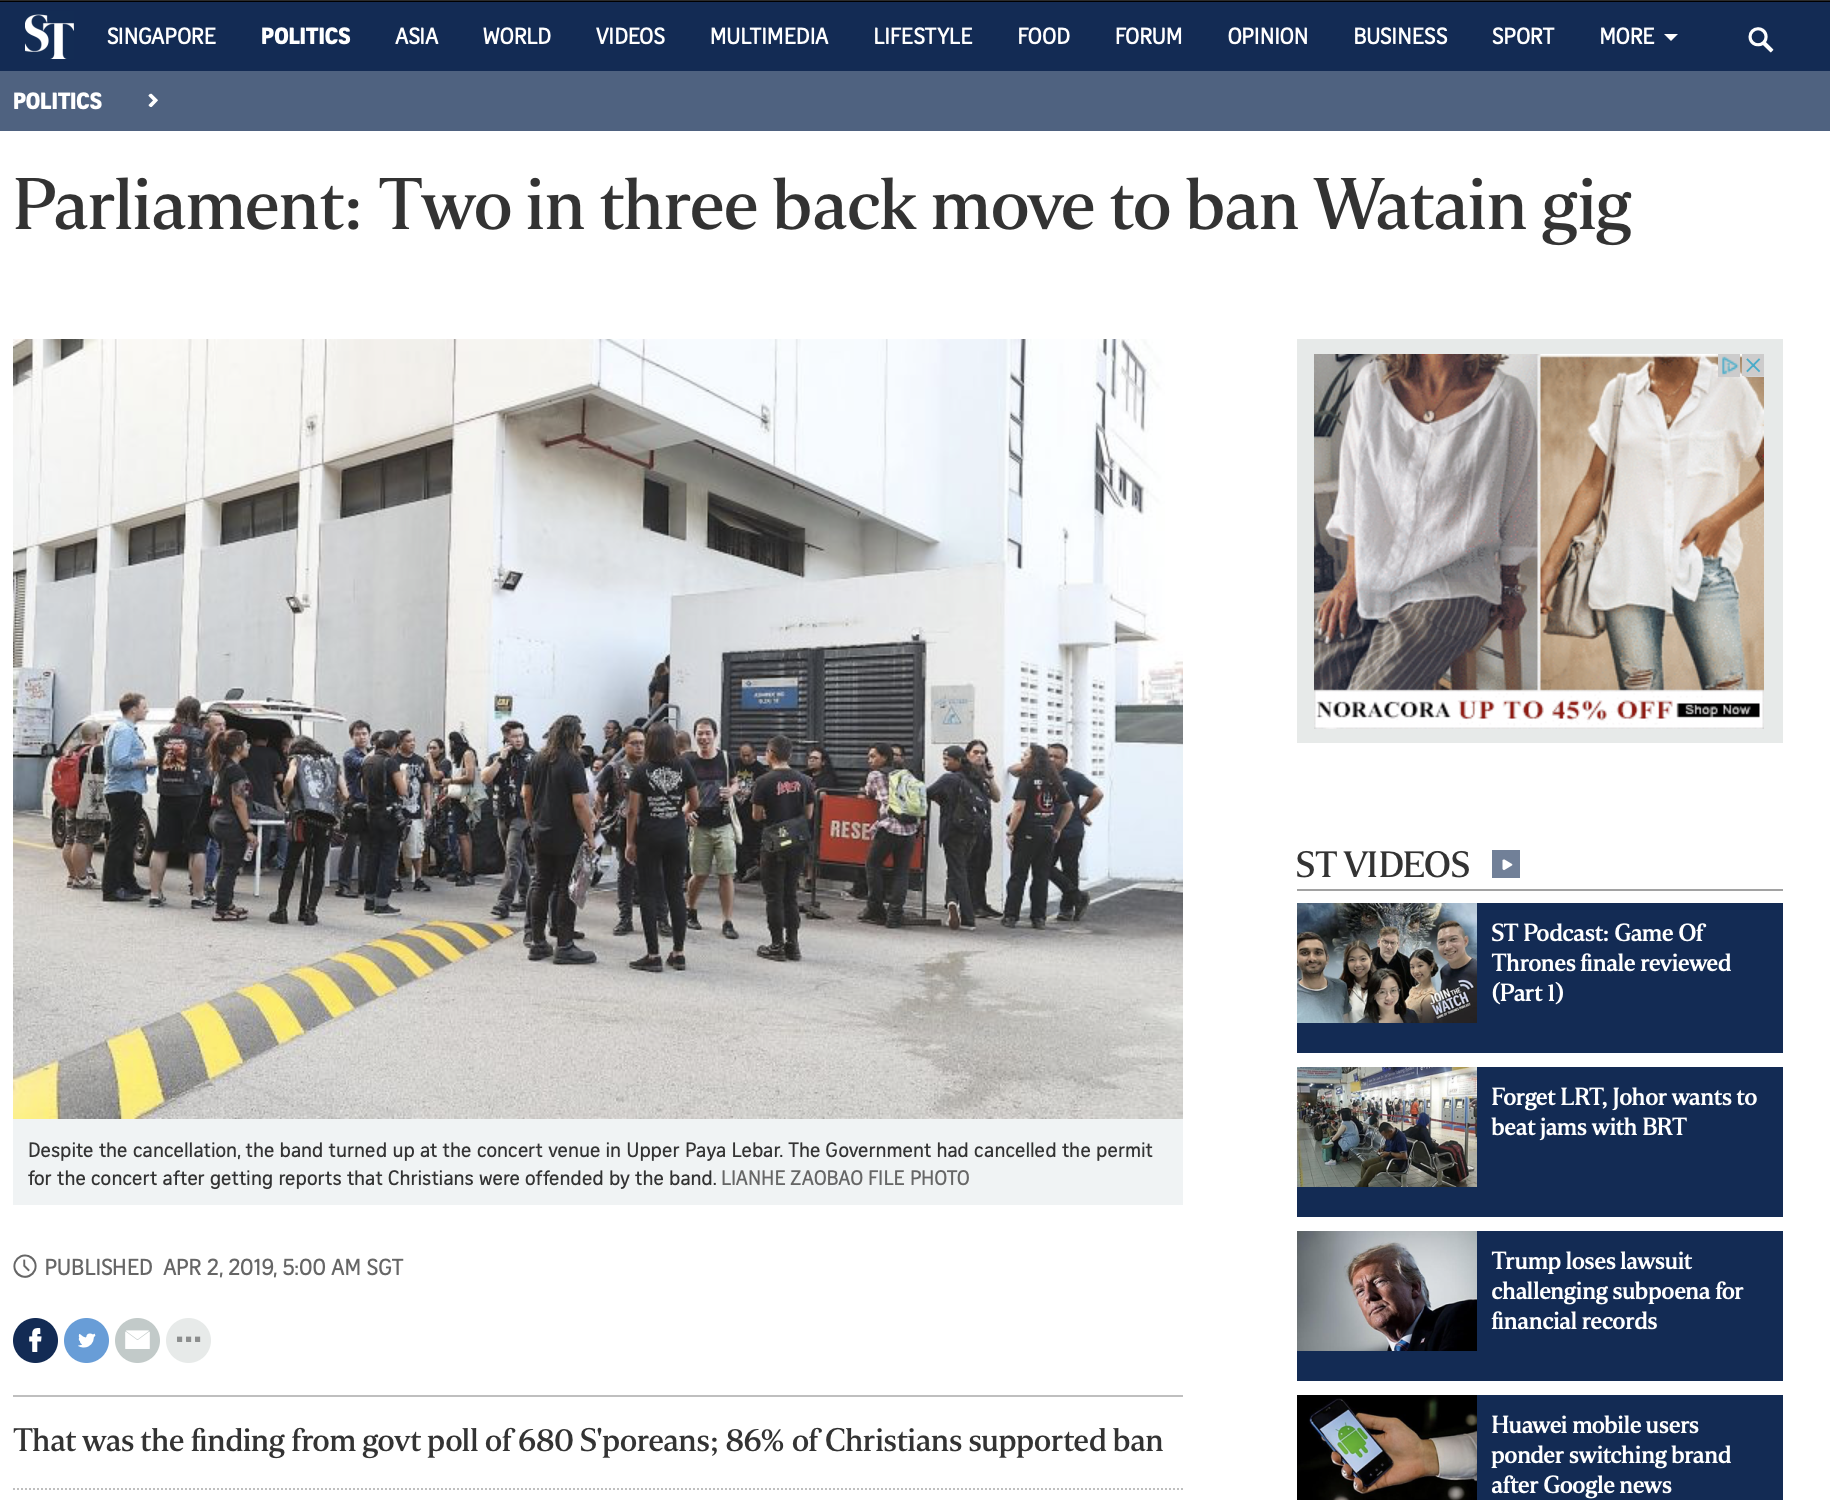
\includegraphics[width=0.8\linewidth]{images/proportion/STwatain} 

}

\caption{Screenshot of online article on results from REACH poll. Retrieved May 21, 2019.}\label{fig:st-watain}
\end{figure}

The next day, national newspaper The Straits Times ran
\href{https://www.straitstimes.com/politics/singapolitics/parliament-two-out-of-three-singaporeans-back-governments-move-to-cancel}{a
story} headlined ``Parliament: Two in three back move to ban Watain
gig''. Within the text of the article, it reads:

\begin{quote}
The Government decided to cancel the permit for Watain's concert last
month when it received reports that mainstream Christians were very
concerned and offended by the band, Home Affairs Minister K. Shanmugam
said yesterday. \textbf{And a survey of Singaporeans by government
feedback unit Reach found that two in three supported the move, he
noted.} Among Christians, 86 per cent were supportive of the move to
disallow the concert, the Reach poll found.
\end{quote}

Note the qualifier ``among those who were aware'' is neither in the
headline (Figure \ref{fig:st-watain}) nor the body of the
article\footnote{CNA ran a similar headline, but included the qualifier
  within the article. See
  \url{https://www.channelnewsasia.com/news/singapore/2-in-3-singaporeans-in-reach-poll-supported-government-s-11401066}}.
\emph{Why is this important?}
\href{https://www.reach.gov.sg/~/media/2019/press-release/findings-of-poll-on-watain-concert--1-april-2019.pdf}{Results
from REACH} show that 63\% of respondents were aware, and \emph{out of
these respondents}, 64\% supported the government's ban. This means that
out of \emph{all} respondents to the survey, only about 40\% reported
supporting the ban. The qualifying phrase ``among those who were aware''
meaningfully changes the interpretation of the results - we shouldn't be
able to say that \textbf{the majority of Singaporeans} supported the ban
when in fact only 40\% of the survey respondents did so.

In effect, the Straits Times article is invoking a strong assumption
here (see \ref{ooptech} for a more technical explanation) - that
\emph{if} those who were unaware were in fact able to express their
support for the ban, the same proportion of respondents (among those who
were aware, 64\%) would also support the ban. But being aware of the ban
is a \emph{prerequisite} for support of the ban, which makes this
assumption rather unreasonable. Even assuming this hypothetical scenario
were possible, the actual figure could be higher or lower - it depends
on how similar (or different) the unaware are to the aware. Those who
were not aware may be less likely to care about black metal music (or
simply too busy to keep up with current affairs) and simply base their
support of the ban on their general sentiment toward government
policies. This seemingly minor omission of the qualifier can lead to
false conclusions pretty quickly. Let us look at another example.

\section{Media claim 2: Web-savvy Seniors}\label{websavvy}

Part of my research involves looking at how Internet use can improve the
lives of older adults \citep[see][]{ang_going_2018}. I was interested in
what the overall situation was like in Singapore, and googled something
like ``internet use seniors''. One 2014 article in the Straits Times
immediately caught my eye (see Figure \ref{fig:st-websavvyseniors}).

\begin{figure}

{\centering 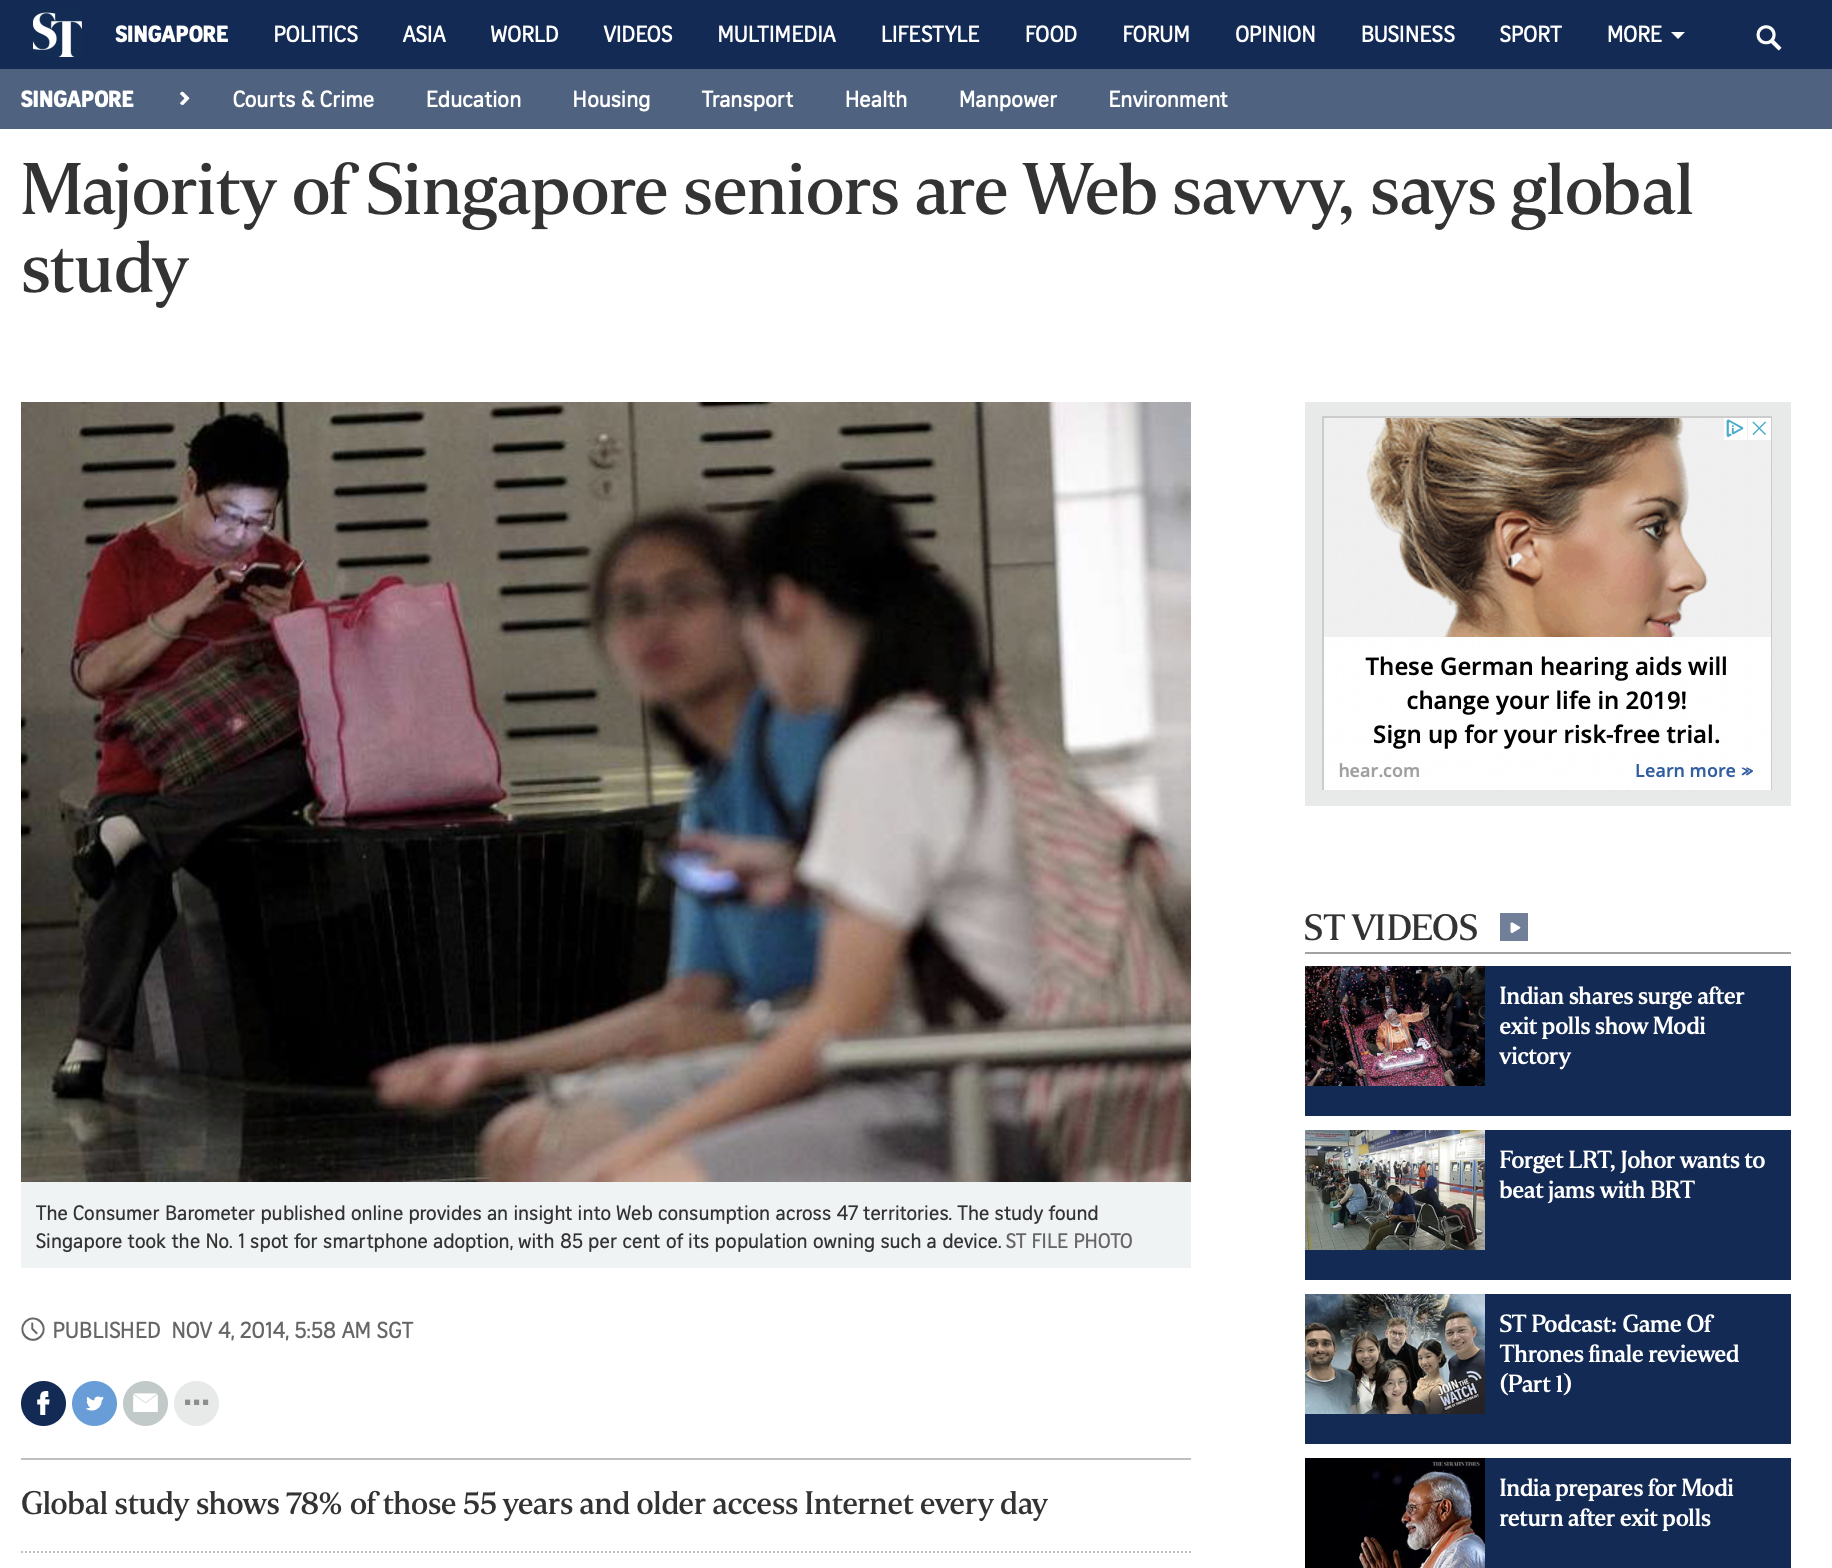
\includegraphics[width=0.8\linewidth]{images/proportion/STwebsavvyseniors} 

}

\caption{Screenshot of online article on web-savvy seniors. Retrieved May 21, 2019.}\label{fig:st-websavvyseniors}
\end{figure}

Within the article, the reporter states:

\begin{quote}
Also, \textbf{78 per cent of those aged 55 and older here access the
Internet every day} either via the traditional Web browser or smartphone
apps, putting Singapore fifth in the world for having the most
Internet-savvy seniors.
\end{quote}

I was skeptical. Over and above my anecdotal experience with Singapore
older adults, past research in the United States\footnote{For instance,
  see
  \url{https://www.pewinternet.org/2012/06/06/older-adults-and-internet-use/}}
gave me reason to expect that the proportion of older people even using
the Internet (everyday or not) should be much lower. Some results from
Consumer Barometer are available online, so we can
\href{https://www.consumerbarometer.com/en/trending/?countryCode=SG\&category=TRN-AGE-55-PLUS}{check
for ourselves}. Of interest in Figure \ref{fig:cb-seniorsinternet} are
numbers reflecting internet use in year 2014, which is when the news
article was published. Note that the percent of Singaporeans aged 55 and
above who use the internet daily in 2014 \textbf{is 29\%, not 78\% as
the article suggests.}

\begin{figure}

{\centering 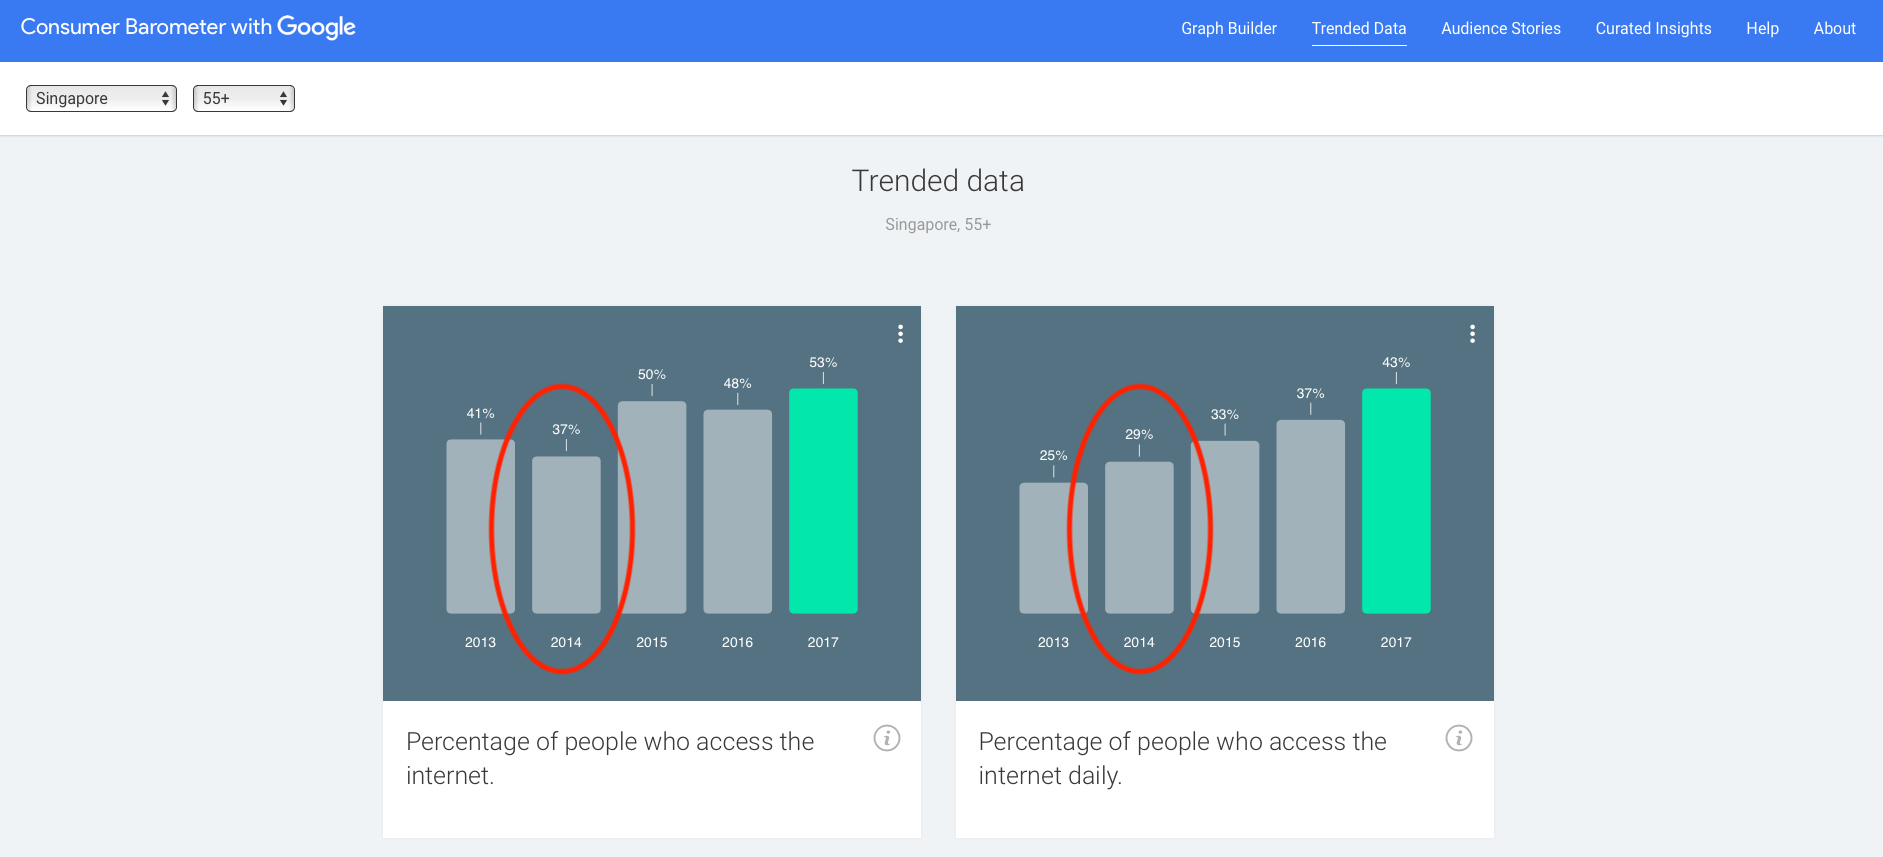
\includegraphics[width=1\linewidth]{images/proportion/CBseniorsinternet} 

}

\caption{Screenshot of Consumer Barometer findings across time. Retrieved May 21, 2019.}\label{fig:cb-seniorsinternet}
\end{figure}

How then, did the reporter get things so wrong? While detailed
statistics for 2014 doesn't seem available online anymore, a little
investigation using 2017 figures shows how the reporter arrived at a
number as high as 78\%.

\begin{figure}

{\centering 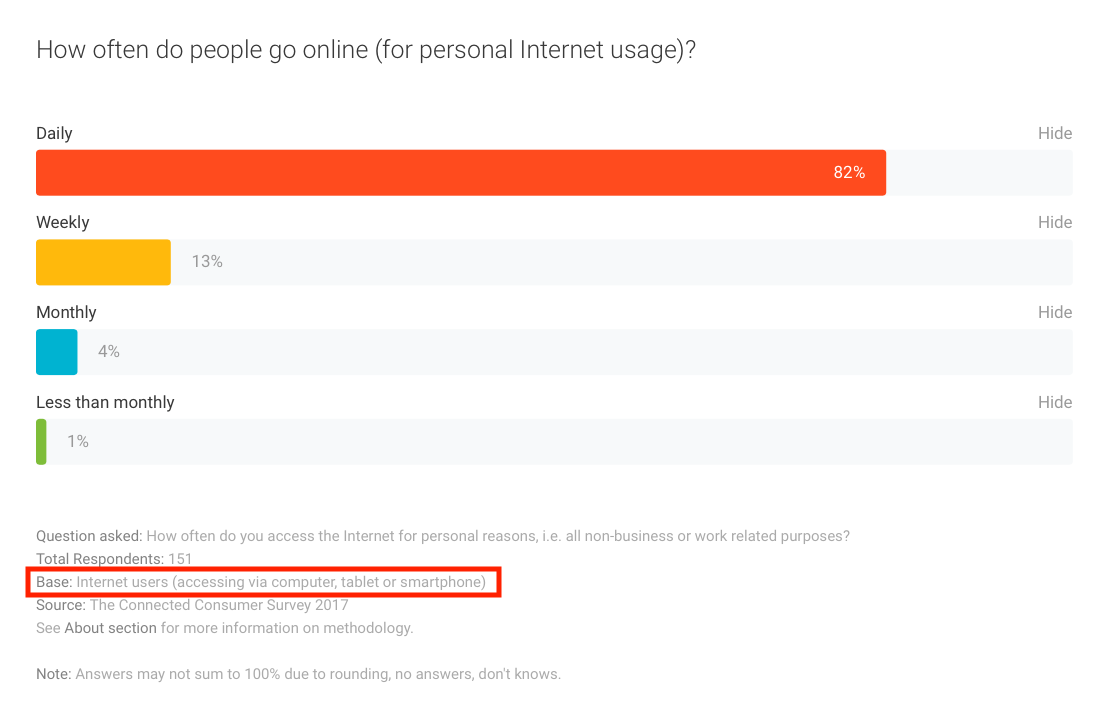
\includegraphics[width=0.9\linewidth]{images/proportion/CBsinglequestion} 

}

\caption{Screenshot of Consumer Barometer results on 2017 internet use. Retrieved May 21, 2019.}\label{fig:cb-single}
\end{figure}

Looking at Figure \ref{fig:cb-single}, the crucial part is the footnote
that says ``base'', which tells us that the 82\% figure for daily
Internet usage in 2017 are \textbf{among those who use the internet}. We
can easily calculate this 82\% with the numbers in Figure
\ref{fig:cb-seniorsinternet} - note that 43\footnote{The percent of
  Singapore residents aged 55+ using the internet in 2017, from Figure
  \ref{fig:cb-seniorsinternet}} is approximately 82\% of 53\footnote{The
  percent of Singapore residents aged 55+ using the internet
  \emph{daily} in 2017, from Figure \ref{fig:cb-seniorsinternet}}. That
is, \(\frac{43}{53} \approx 0.82\). This recovers the 82\% figure that
we see in Figure \ref{fig:cb-single}.

Using the same strategy, we can recover the reporter's figure for 2014:
\(\frac{29}{37} \approx 0.78\).

\emph{What does this mean?} This means that just like the reporter in
the Watain example (\ref{watain}), this reporter left out an important
qualifier - only 29\% of all older adults in Singapore use the internet
daily, but 78\% \textbf{of those who use the internet} use it daily.
This vast discrepancy is highly consequential - the statement that ``78
per cent of those aged 55 and older here access the Internet every day''
is false, and the headline that ``Majority of Singapore seniors are Web
savvy'' is misleading at best.

\section{Technical excursus}\label{ooptech}

Before we go into a more technical explanation of what went wrong in
these two cases, let us first move from proportions to probabilities.
The difference between a proportion and a probability is important here.
Note that when Minister Shanmugam asserted the REACH poll provided
evidence that the Government's ``assessment of public sentiment turned
out to be correct'', he was not suggesting that 680 Singaporeans form
the whole Singapore public. The underlying assumption was that since
most survey respondents (who were aware) supported the ban, it is likely
that most Singaporeans (who are aware) will also support the ban. That
is, he was using the \emph{proportion} of supportive survey respondents
(a description of the sample), to infer the \emph{probability} (a
hypothetical quantity) of any one Singaporean supporting the ban.

The difference between a probability and a proportion may be simplified
using a coin flip example. If I flip a fair coin 4 times, the proportion
of heads may be 0, 0.25, 0.5, 0.75, or 1. However, since it is a fair
coin, the probability of getting a heads is, by definition, 0.5. So the
proportion may or may not equal the probability. What we know is that
the more times I flip the coin, the more likely the proportion of heads
will reflect the true probability of getting a heads. It is thus common
to hear people say that the probability is the ``long-run proportion of
an event''. Below is some code (in R) for you to try out the coin flip
example.

\begin{Shaded}
\begin{Highlighting}[]
\CommentTok{# Set the number of trials to 4. }
\CommentTok{# You may change the number to see what happens.}
\NormalTok{n <-}\StringTok{ }\DecValTok{4} 
\CommentTok{# Get the proportion of heads after flipping a fair coin n times. }
\CommentTok{# Try this a few times.}
\KeywordTok{sum}\NormalTok{(}\KeywordTok{rbinom}\NormalTok{(n, }\DecValTok{1}\NormalTok{, }\DataTypeTok{prob=}\FloatTok{0.5}\NormalTok{))}\OperatorTok{/}\NormalTok{n }
\end{Highlighting}
\end{Shaded}

We have now established that the main reason why we are interested in
proportions from a REACH poll is because they purport to tell us
something about Singaporeans in general. That is, the REACH poll
suggests that if we were to randomly pick a Singaporean from those who
are aware of the ban, the probability of this person supporting the ban
is about 0.64 (or 64\%). The problem at hand then reduces to a trivial
probability question, assuming that we all remember basic probability
rules from secondary (primary?) school\footnote{Or that we can Google it
  if not}. If the REACH poll is indeed representative of all
Singaporeans, then we have the following quantities:

 \[
\begin{aligned}
&\Pr(\text{Aware of Ban}) = 0.63 \\
&\Pr(\text{Not Aware of Ban}) = 1 - \Pr(\text{Aware of Ban}) = 0.37 \\
&\Pr(\text{Support Ban } | \text{ Aware of Ban}) = 0.64 
\end{aligned}
\]

\(\Pr(\text{Support Ban } | \text{ Aware of Ban})\) is a conditional
probability, but the quantity that is being asserted in the news article
is \(\Pr(\text{Support Ban})\), which is the total probability. Using
the law of total probability, we know that:

 \[
\begin{aligned}
\Pr(\text{Support Ban}) &= \Pr(\text{Support Ban } | \text{ Aware of Ban})\cdot \Pr(\text{Aware of Ban}) \\
& \quad + \Pr(\text{Support Ban } | \text{ Not Aware of Ban})\cdot \Pr(\text{Not Aware of Ban}) 
\end{aligned}
\]

Plugging in the numbers that we have,

 \[
\begin{aligned}
\Pr(\text{Support Ban}) &= 0.64 \cdot 0.63 + \Pr(\text{Support Ban } | \text{ Not Aware of Ban}) \cdot 0.37 \\
\end{aligned}
\]

we see that \(\Pr(\text{Support Ban}) = 0.64\) if and only if
\(\Pr(\text{Support Ban } | \text{ Not Aware of Ban})\) also equals
\(0.64\). That said,
\(\Pr(\text{Support Ban } | \text{ Not Aware of Ban})\) is logically
impossible, and should equal zero. Similarly, for the Web-savvy Seniors
example,

 \[
\begin{aligned}
\Pr(\text{Use Internet Daily}) &= \Pr(\text{Use Internet Daily } | \text{ Use Internet})\cdot \Pr(\text{Use Internet}) \\
& \quad + \Pr(\text{Use Internet Daily } | \text{ Don't Use Internet})\cdot \Pr(\text{Don't Use Internet}) \\
&= 0.78 \cdot 0.37 + \Pr(\text{Use Internet Daily } | \text{ Don't Use Internet})\cdot 0.63 \\
\end{aligned}
\]

where \(\Pr(\text{Use Internet Daily } | \text{ Don't Use Internet})\)
is impossible and should be zero. In both cases, total probabilites are
substantially different from the conditional probabilities, and there is
no reason to believe they would be the same.

\section{Conclusion}\label{conclusion}

By now, it should be clear that qualifiers attached to proportions (and
percentages) are critical. Without them, results from studies can be
blown out of proportion. It is not wise to completely rely on assertions
made by news articles (or other kinds of reports), even from supposedly
credible agencies like the Straits Times. As we have seen, social
scientists should be comfortable with interpreting data from its
source\footnote{This, however, first requires data to be made available
  for replication purposes.} in order to evaluate claims that are being
made in public discourse today.

\section{Additional reading}\label{additional-reading}

Straits Times reporter Christopher Tan alleges (July 5, 2019) that the
Land Transport Authority also makes this kind of misleading
representation of support for legalizing onboard audio recordings in
taxis and private hire cars: See
\url{https://www.straitstimes.com/opinion/recording-in-taxis-for-hire-cars-consider-cost-consequences}.
You may want to check the source material
\href{https://www.lta.gov.sg/apps/news/page.aspx?c=2\&id=6157ec3f-4e45-4dcc-9c78-7d8506084576\#2}{from
LTA} and
\href{https://www.reach.gov.sg/~/media/2019/press-release/invehicle-recording-devices-poll-media-release.pdf}{REACH}
to judge for yourself if he is correct.

\chapter{Are we lonely?}\label{lonely}

\begin{verbatim}
Contributor: Shannon Ang
Date: 25 May 2019
\end{verbatim}

In population health research, there are a number of commonly used
scales to measure psychosocial well-being. For instance, the
\href{https://www.apa.org/pi/about/publications/caregivers/practice-settings/assessment/tools/depression-scale}{Center
for Epidemiologic Studies Depression Scale} (CES-D) is widely used to
measure depression, and the
\href{https://euroqol.org/eq-5d-instruments/}{EQ-5D}\footnote{There's no
  `full' name for this, its just referred to as the EQ-5D.} to measure
quality of life. These scales seldom have an intuitive interpretation -
who knows what 10 points on the CES-D scale actually means in `real
life', versus 12 points? To address this, social scientists often choose
a ``cut-off'' point to simplify the measure into two categories (e.g.,
either you are depressed, or you are not). Some of these cut-off points
are well researched (such the cut-off point for mild cognitive
impairment), while others are more arbitrary.

This case study looks at the prevalence of loneliness in Singapore older
adults, and how these cut-offs can shape the way we think about it. The
focus here is \emph{not} to criticize researchers' choices of cut-off
points. Instead, this case study seeks to provide a way to evaluate
claims that are based on these cut-offs, so that we understand how to
compare claims across studies and/or reports.

\section{The lonely dichotomy}\label{the-lonely-dichotomy}

Loneliness is a real issue for many people today, and it has been shown
to have deleterious effects on health
\citep{rico-uribe_association_2018}. More of us are beginning to realize
that social connections are key, especially for older persons. The
Straits Times carried an
\href{https://www.straitstimes.com/singapore/living-with-family-but-still-feeling-lonely}{article}
in 2018, with the headline ``Senior citizens living with family, but
still feeling lonely''.

\begin{figure}

{\centering 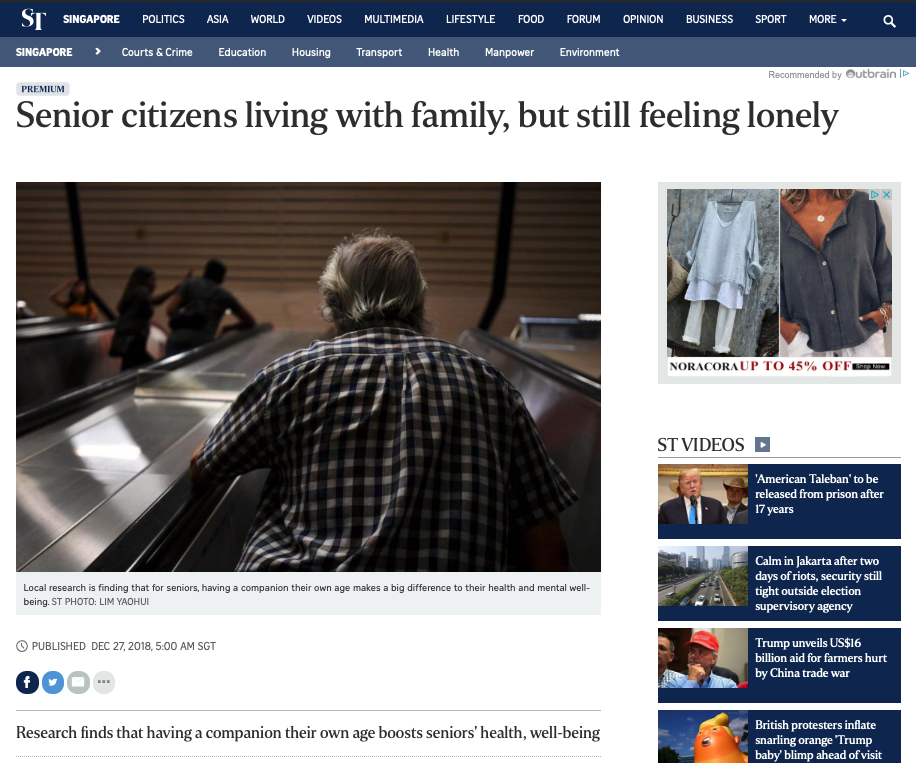
\includegraphics[width=0.8\linewidth]{images/loneliness/livingarr} 

}

\caption{Screenshot of online article on lonely seniors. Retrieved May 25, 2019.}\label{fig:st-lonely}
\end{figure}

But what does \textbf{feeling lonely} really mean? There seems to be a
dichotomy being drawn here - either you feel lonely, or you don't feel
lonely. There is little room for nuance like ``I feel lonely when I ride
the bus by myself''. Of course, some level of simplification is needed
to compare across groups - and this simplification is what we need to
examine.

The news article highlights studies on loneliness (in Singapore) done by
two different groups - a team at the National Healthcare Group (NHG),
and a team at the Centre for Ageing Research and Education (CARE) in
Duke-NUS Medical School\footnote{Led by Associate Professor
  \href{https://www.duke-nus.edu.sg/hssr/our-team/faculty/faculty-staff-details/Detail/13200}{Angelique
  Chan}}. As we will see, this lonely/not lonely dichotomy is drawn by
reseachers as well, but sometimes \textbf{in completely different ways}.
Let us take a closer look.

\section{Lonely by whose standard}\label{lonely-by-whose-standard}

The studies of interest\footnote{All these studies are open-access
  articles, anyone can access them even without a library subscription.}
here are \citet{wee_loneliness_2019}, \citet{ge_social_2017},
\citet{lim_association_2017}, and \citet{chan_loneliness_2015}. All of
these studies use a variant of the 3-item UCLA\footnote{University of
  California, Los Angeles} Loneliness Scale \citep{hughes_short_2004}.
The 3-item UCLA Loneliness Scale consists of three questions, which all
of these studies use:

\begin{enumerate}
\def\labelenumi{\arabic{enumi}.}
\tightlist
\item
  How often do you feel you lack companionship?
\item
  How often do you feel left out?
\item
  How often do you feel isolated from others?
\end{enumerate}

For each of the questions listed above, respondents were given a range
of responses to choose from. These are listed in Figure
\ref{fig:st-lonely-graph}. As you might notice, they were different
across the studies. \citet{wee_loneliness_2019} and
\citet{ge_social_2017} had only 3 response categories (the right
column), while \citet{lim_association_2017} and
\citet{chan_loneliness_2015} had 5 different response categories (the
left column). I put the point values for each response in parentheses.
In all of these studies, researchers added up these points across the 3
questions, and came up with their own `cut-off' point to determine who
was ``lonely''.

\begin{figure}

{\centering 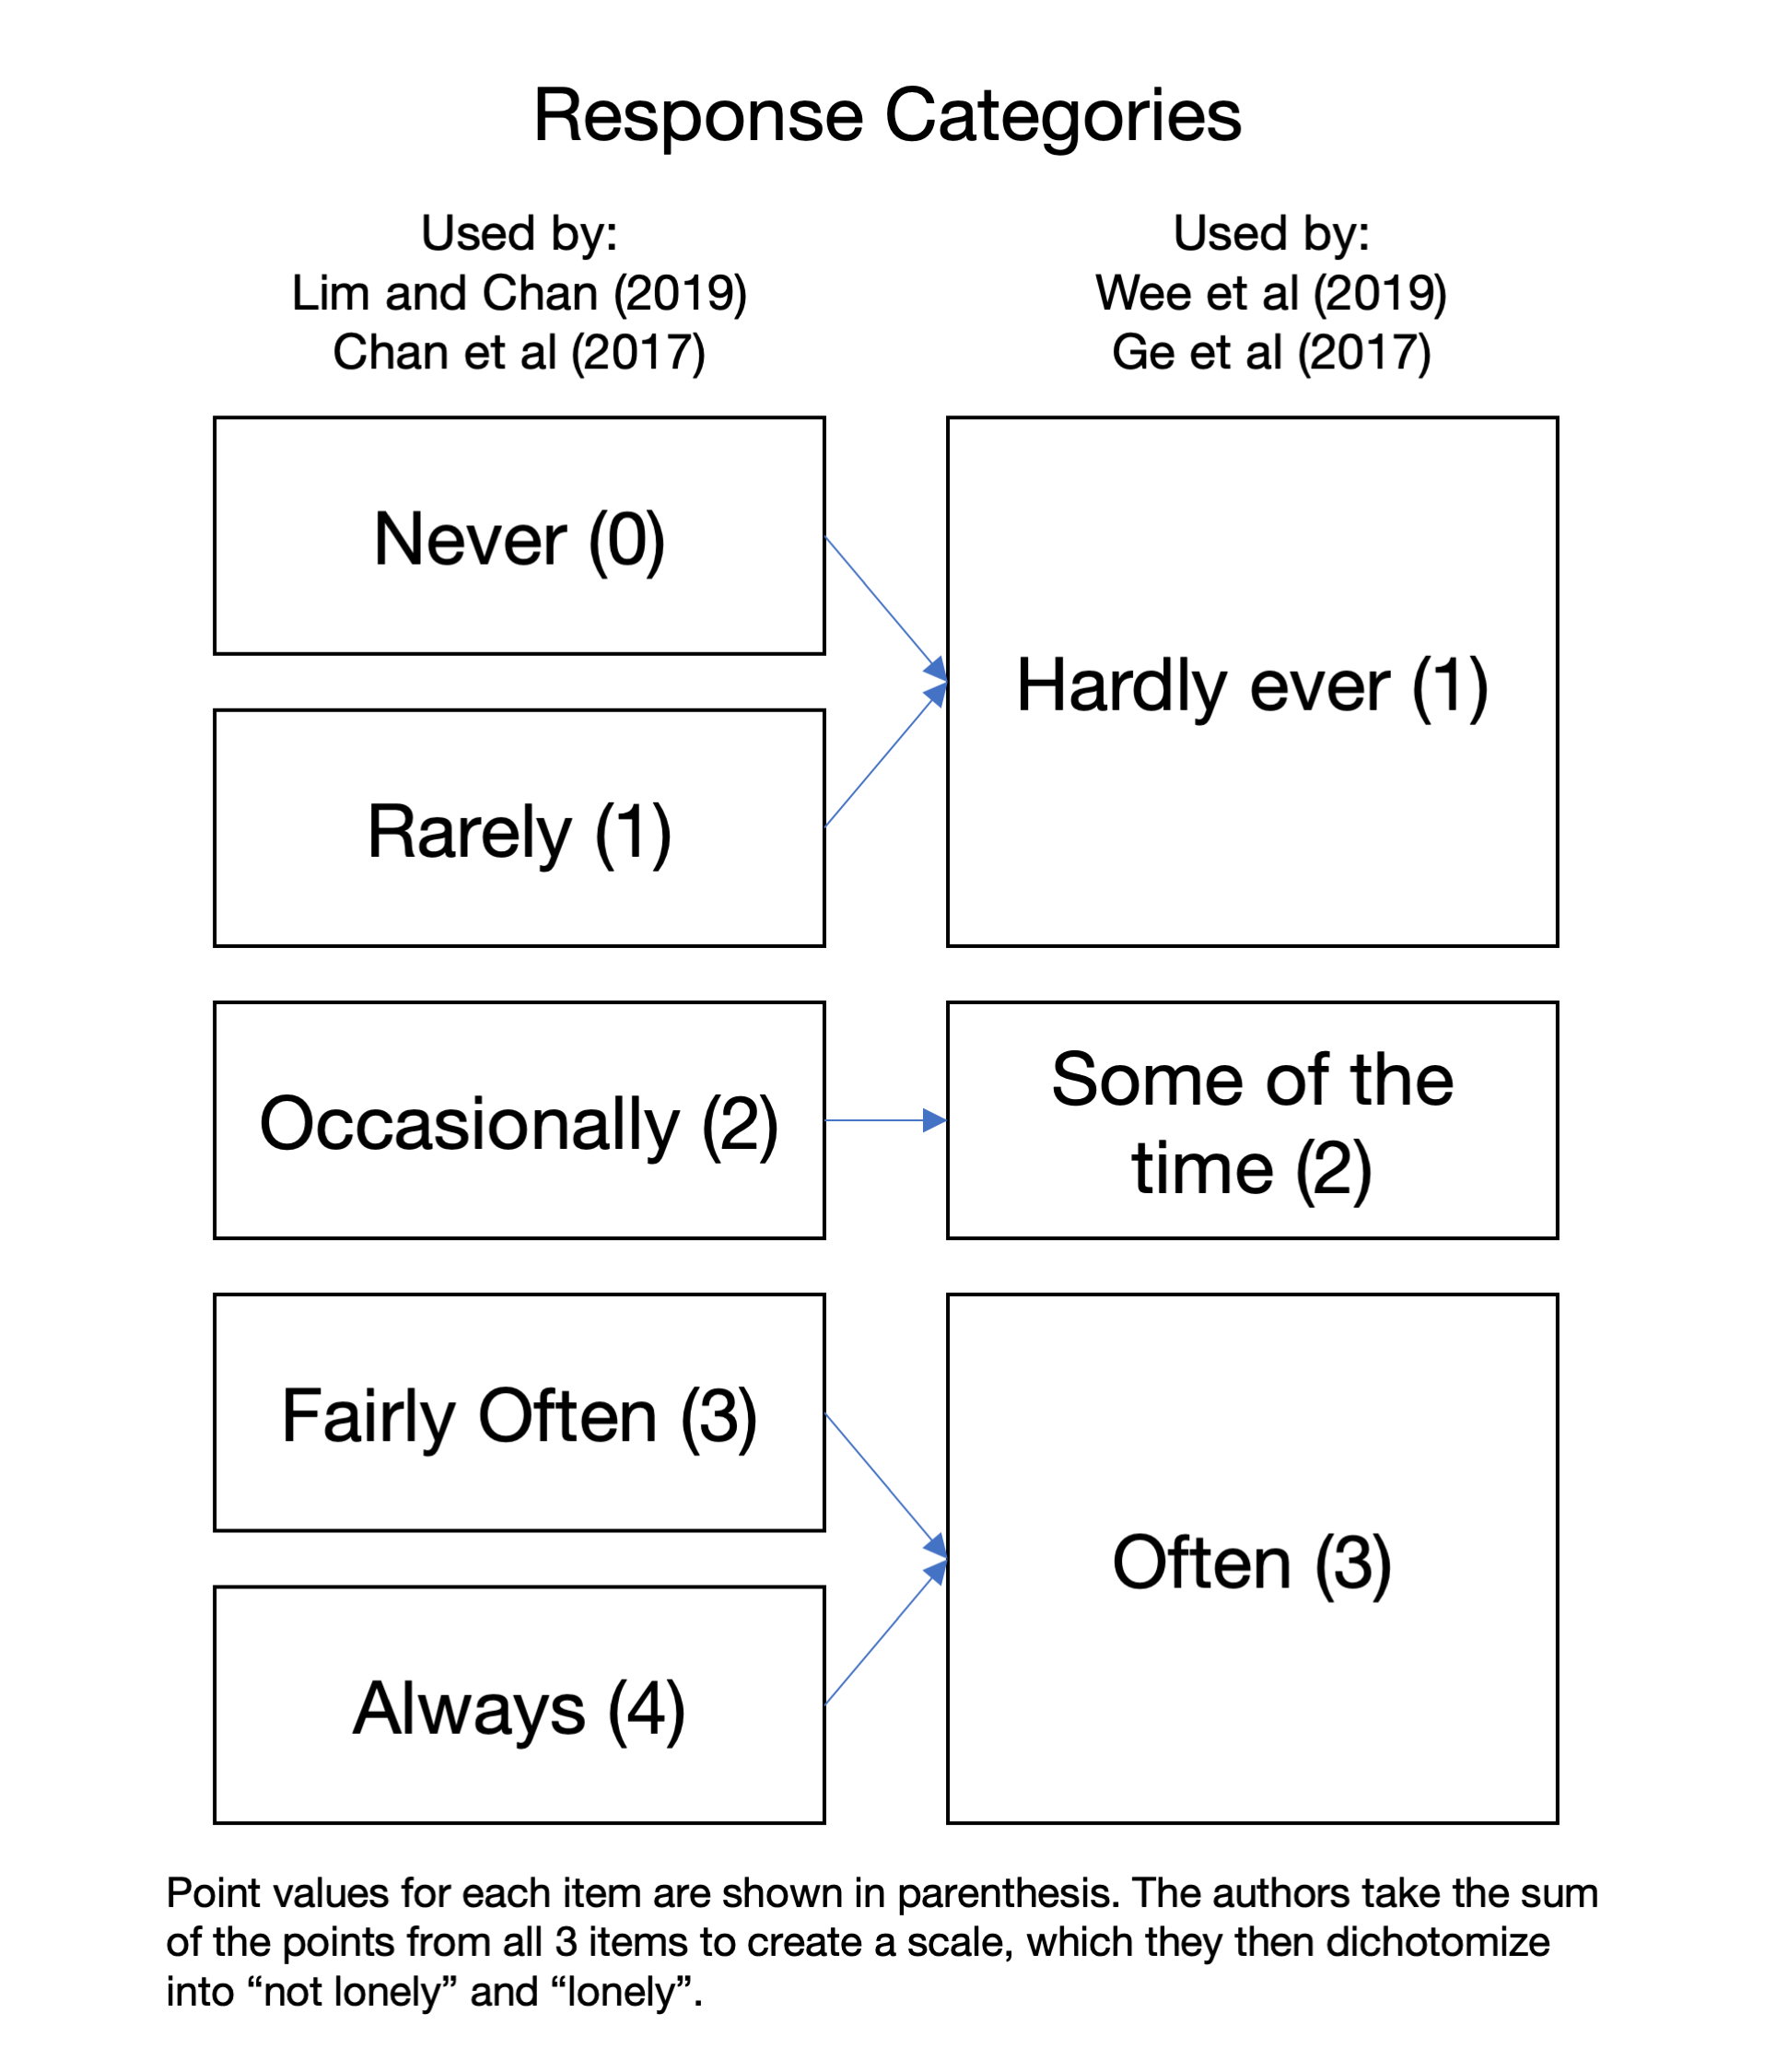
\includegraphics[width=0.5\linewidth]{images/loneliness/lonely_graph} 

}

\caption{Summary of response categories}\label{fig:st-lonely-graph}
\end{figure}

I added the \textbf{blue arrows} in Figure \ref{fig:st-lonely-graph} to
show how the 5 category option can be mapped to the 3 category option
(but not vice versa). We don't really know what kind of bias this will
introduce\footnote{For instance, one might argue that respondents might
  choose differently when given more gradational categories.}, but at
face value I think this looks pretty reasonable. Why am I doing this?
This ``matching'' allows us to do a little experiment with publicly
available data\footnote{So you can try it yourself} to answer the
following question: \textbf{How does changing the criteria change our
view of loneliness in Singapore?} The next section compares these
different coding schemes.

\section{Same data, different
results}\label{same-data-different-results}

For this simple analysis, I use data from Wave 2 of the Panel on Health
and Ageing of Singaporean Elderly (PHASE) (see \ref{phase}), conducted
in 2011. This is a nationally representative study of older adults aged
60 and above. It is essentially the same dataset used in
\citet{lim_association_2017} and \citet{chan_loneliness_2015}. Code
provided is in R. For the sake of brevity, I leave out observations with
any missing values on any of the loneliness items. A key concern of the
news article in Figure \ref{fig:st-lonely} is that even older adults
living with family members may be lonely, so we will look at a
cross-tabulation of living arrangements with ``loneliness''.

\textbf{Coding scheme 1: Lots of loneliness}

I first follow the coding scheme in \citet{lim_association_2017} and
\citet{chan_loneliness_2015}. I sum the items up (giving me a score that
ranges from 0-12), and then dichotomize respondents into people who are
``not lonely'' (score of 0), and those who are ``lonely'' (score of
1-12)\footnote{Note that \citet{chan_loneliness_2015} further splits the
  ``lonely'' group into ``sometimes lonely'' and ``mostly lonely''.
  \citet{lim_association_2017}, however, does not make this distinction.
  I have grouped them together since this is the way that it has usually
  been represented in public discourse (e.g., the claim that those who
  are lonely have a higher risk of mortality compared to those not
  lonely. See, for instance,
  \url{https://www.straitstimes.com/singapore/those-who-feel-lonely-more-prone})}.
This cut-off point seems to have arisen from a ``common-sense'' approach
rather than any kind of formal testing - that is, group the people who
never experience loneliness in one group, and then put the rest who have
had some experience of loneliness in another.

\begin{Shaded}
\begin{Highlighting}[]
\CommentTok{# Load required libraries}
\KeywordTok{library}\NormalTok{(dplyr)}
\end{Highlighting}
\end{Shaded}

\begin{Shaded}
\begin{Highlighting}[]
\CommentTok{# Note: You first need to read in the data}
\CommentTok{# The data already contains a pre-coded version according to these criteria}
\NormalTok{lonely1_cat <-}\StringTok{ }\NormalTok{phase}\OperatorTok{$}\NormalTok{w2_loneliness_yesno }\OperatorTok
\StringTok{  }\KeywordTok{factor}\NormalTok{(}\DataTypeTok{labels=}\KeywordTok{c}\NormalTok{(}\StringTok{"Not lonely"}\NormalTok{, }\StringTok{"Lonely"}\NormalTok{))}
\CommentTok{# Make a table (proportions are weighted to account for survey design)}
\NormalTok{knitr}\OperatorTok{::}\KeywordTok{kable}\NormalTok{(}
\NormalTok{  GDAtools}\OperatorTok{::}\KeywordTok{prop.wtable}\NormalTok{(livingarr, lonely1_cat, }
                      \DataTypeTok{dir=}\DecValTok{1}\NormalTok{, }\DataTypeTok{digits=}\DecValTok{3}\NormalTok{, }\DataTypeTok{w=}\NormalTok{phase}\OperatorTok{$}\NormalTok{w2_weights, }\DataTypeTok{na=}\NormalTok{F, }\DataTypeTok{mar=}\NormalTok{F), }
  \DataTypeTok{caption =} \KeywordTok{paste0}\NormalTok{(}\StringTok{'Crosstabulation using criteria in Lim and Chan (2017) '}\NormalTok{,}
                   \StringTok{'and Chan et al (2015). Note that these are row percentages.'}\NormalTok{),}
  \DataTypeTok{booktabs =} \OtherTok{TRUE}\NormalTok{)}
\end{Highlighting}
\end{Shaded}

\begin{table}

\caption{\label{tab:table-lonely1}Crosstabulation using criteria in Lim and Chan (2017) and Chan et al (2015). Note that these are row percentages.}
\centering
\begin{tabular}[t]{lrr}
\toprule
  & Not lonely & Lonely\\
\midrule
Living alone & 41.022 & 58.978\\
Living with spouse only & 67.844 & 32.156\\
Living with child only & 49.910 & 50.090\\
Living with spouse and child & 71.680 & 28.320\\
Living with others only & 44.791 & 55.209\\
\bottomrule
\end{tabular}
\end{table}

Table \ref{tab:table-lonely1} gives me a similar proportion as suggested
in the news article - that is,

\begin{quote}
``{[}Associate Professor Chan's study{]} found that half of Singaporeans
over 60 felt lonely some or most of the time. But those who lived with
spouses, or with spouses and children, did not.''
\end{quote}

 These numbers are indeed worrying. Older adults living alone are
understandably lonely, but those who live with their children (but
without their spouse) are not that far behind (50.1\%!). Even 28\% of
those who live with their spouse and child feel lonely, like the
headline in the news article (Figure \ref{fig:st-lonely}) suggests.

\textbf{Coding scheme 2: Not that much loneliness}

We then arrive at the coding scheme used by \citet{wee_loneliness_2019}
and \citet{ge_social_2017}. Summing the items gives me a score that
ranges from 3-9, and I then dichotomize the group into people who are
``not lonely'' (score of 3-5), and those who are ``lonely'' (score of
6-9). Note that these cut-points are probably arbitrary - while the
researchers cite a paper each to justify their use of the cut-point, the
cited papers do not really provide evidence in support of the cut-point.
The closest support for the cut-point in the cited papers that I could
discern is in \citet{steptoe_social_2013}, which states that they used
the top quintile\footnote{In their sample, not the Singapore one.} to
define loneliness. No reason was given as to why the top quintile was
chosen. Table \ref{tab:table-lonely2} shows the distribution of
``loneliness'' according to these criteria.

\begin{Shaded}
\begin{Highlighting}[]
\CommentTok{# Recode and sum the loneliness scores}
\NormalTok{lonely2 <-}\StringTok{ }\NormalTok{phase }\OperatorTok\StringTok{ }
\StringTok{  }\KeywordTok{select}\NormalTok{(w2_Q10_1_GV1, w2_Q10_2_GV1, w2_Q10_3_GV1) }\OperatorTok\StringTok{  }
\StringTok{  }\KeywordTok{mutate_all}\NormalTok{(}\KeywordTok{funs}\NormalTok{(}\KeywordTok{recode}\NormalTok{(.,}\StringTok{`}\DataTypeTok{0}\StringTok{`}\NormalTok{ =}\StringTok{ }\DecValTok{1}\NormalTok{, }\StringTok{`}\DataTypeTok{1}\StringTok{`}\NormalTok{ =}\StringTok{ }\DecValTok{1}\NormalTok{, }\StringTok{`}\DataTypeTok{2}\StringTok{`}\NormalTok{ =}\StringTok{ }\DecValTok{2}\NormalTok{, }\StringTok{`}\DataTypeTok{3}\StringTok{`}\NormalTok{ =}\StringTok{ }\DecValTok{3}\NormalTok{, }\StringTok{`}\DataTypeTok{4}\StringTok{`}\NormalTok{ =}\StringTok{ }\DecValTok{3}\NormalTok{))) }\OperatorTok
\StringTok{  }\KeywordTok{rowSums}\NormalTok{()}

\CommentTok{# Categorize according to cut-off point}
\NormalTok{lonely2_cat <-}\StringTok{ }\KeywordTok{if_else}\NormalTok{(lonely2 }\OperatorTok{<}\StringTok{ }\DecValTok{6}\NormalTok{, }\DecValTok{0}\NormalTok{, }\DecValTok{1}\NormalTok{) }\OperatorTok\StringTok{ }
\StringTok{  }\KeywordTok{factor}\NormalTok{(}\DataTypeTok{labels=}\KeywordTok{c}\NormalTok{(}\StringTok{"Not lonely"}\NormalTok{, }\StringTok{"Lonely"}\NormalTok{))}

\CommentTok{# Show table}
\NormalTok{knitr}\OperatorTok{::}\KeywordTok{kable}\NormalTok{(}
\NormalTok{  GDAtools}\OperatorTok{::}\KeywordTok{prop.wtable}\NormalTok{(livingarr, lonely2_cat, }
                      \DataTypeTok{dir=}\DecValTok{1}\NormalTok{, }\DataTypeTok{digits=}\DecValTok{3}\NormalTok{, }\DataTypeTok{w=}\NormalTok{phase}\OperatorTok{$}\NormalTok{w2_weights, }\DataTypeTok{na=}\NormalTok{F, }\DataTypeTok{mar=}\NormalTok{F), }
  \DataTypeTok{caption =} \KeywordTok{paste0}\NormalTok{(}\StringTok{'Crosstabulation using criteria in Wee et al (2019) '}\NormalTok{,}
            \StringTok{'and Ge et al (2017). Note that these are row percentages.'}\NormalTok{),}
  \DataTypeTok{booktabs =} \OtherTok{TRUE}\NormalTok{)}
\end{Highlighting}
\end{Shaded}

\begin{table}

\caption{\label{tab:table-lonely2}Crosstabulation using criteria in Wee et al (2019) and Ge et al (2017). Note that these are row percentages.}
\centering
\begin{tabular}[t]{lrr}
\toprule
  & Not lonely & Lonely\\
\midrule
Living alone & 84.419 & 15.581\\
Living with spouse only & 96.555 & 3.445\\
Living with child only & 92.184 & 7.816\\
Living with spouse and child & 97.863 & 2.137\\
Living with others only & 93.046 & 6.954\\
\bottomrule
\end{tabular}
\end{table}

What you will immediately realize is that these numbers are way lower
than those when using coding scheme 1 (that is, the coding scheme of
\citet{lim_association_2017} and \citet{chan_loneliness_2015}). These
numbers are more consistent with the figures shown in
\citet{ge_social_2017}\footnote{Note that the sample in
  \citet{ge_social_2017} is of all adults aged 21 and older, not just
  older adults, so the higher number seen here is expected. Note also
  that in the paper, the authors show column percentages instead of row
  percentages. Since we are comparing across living arrangements
  however, row percentages are more appropriate.}. Further, the
difference in the proportion of those living alone and those living with
their child (but without their spouse) is similar in absolute terms, but
much larger in relative terms (see Table \ref{tab:table-lonely3}). While
the proportion of those lonely among those who live alone is 1.2 times
that of those living with only their children according to coding scheme
1, this ratio increases to 2 when using coding scheme 2. Based on these
results, it seems that the overall loneliness situation is much less
dire than before, and those who live with children don't seem as
isolated as those who live alone after all.

\begin{table}

\caption{\label{tab:table-lonely3}Comparison of absolute and relative differences}
\centering
\begin{tabular}[t]{lrr}
\toprule
  & Coding scheme 1 & Coding scheme 2\\
\midrule
(1) Living alone & 59.0 & 15.6\\
(2) Living with child only & 50.1 & 7.8\\
Difference [(1) - (2)] & 8.9 & 7.8\\
Ratio [(1)/(2)] & 1.2 & 2.0\\
\bottomrule
\end{tabular}
\end{table}

\section{Conclusion}\label{conclusion-1}

You may be thinking, so which way of conceptualizing loneliness is
``correct''? As I mentioned at the start of this case study, that is not
the goal here. The process of figuring out a useful cut-off point is a
long and tedious one that requires researchers to engage with each
other\footnote{And indeed, Singapore social science can perhaps use more
  of this.}. Rather, the goal here has been to highlight that decisions
like cut-off points may seem small, but are critical in the way we
interpret and talk about social phenomena. In this case study, these
cut-off points essentially define who is considered lonely. \textbf{If
these cut-off points are vastly different, we may not be even talking
about the same people} when we talk about ``lonely persons''. This means
that when comparing or drawing conclusions from the findings of
different studies, it is crucial that we understand the decisions that
produced the numbers.

\chapter{Size is not all that matters}\label{samples}

\begin{verbatim}
Contributor: Shannon Ang
Date: 22 July 2019
\end{verbatim}

In response to public surveys, it's quite common to hear people make
comments like ``they asked only 1000 people, how accurate can it be?''.
Of course, people tend to only say these things when the findings
presented are incongruent with their perception of reality.

This case study looks at whether and how size makes a difference when
we're trying to understand survey results from samples of the
population. My hope is for you (the reader) to realize that often,
\emph{how} the sample is drawn (and how we quantify uncertainty) is more
important than the size of the sample.

\section{But it's too small!}\label{sample-worklife}

We will first look at an example. Local newspaper The Straits Times
recently reported the findings of a
\href{https://www.michaelpage.com.sg/advice/career-advice/work-life-balance/singapore-happy-work}{study
done by Michael Page}, alleging that \textbf{8 of out 10 people are
``happy'' with their work-life balance}.

\begin{figure}

{\centering 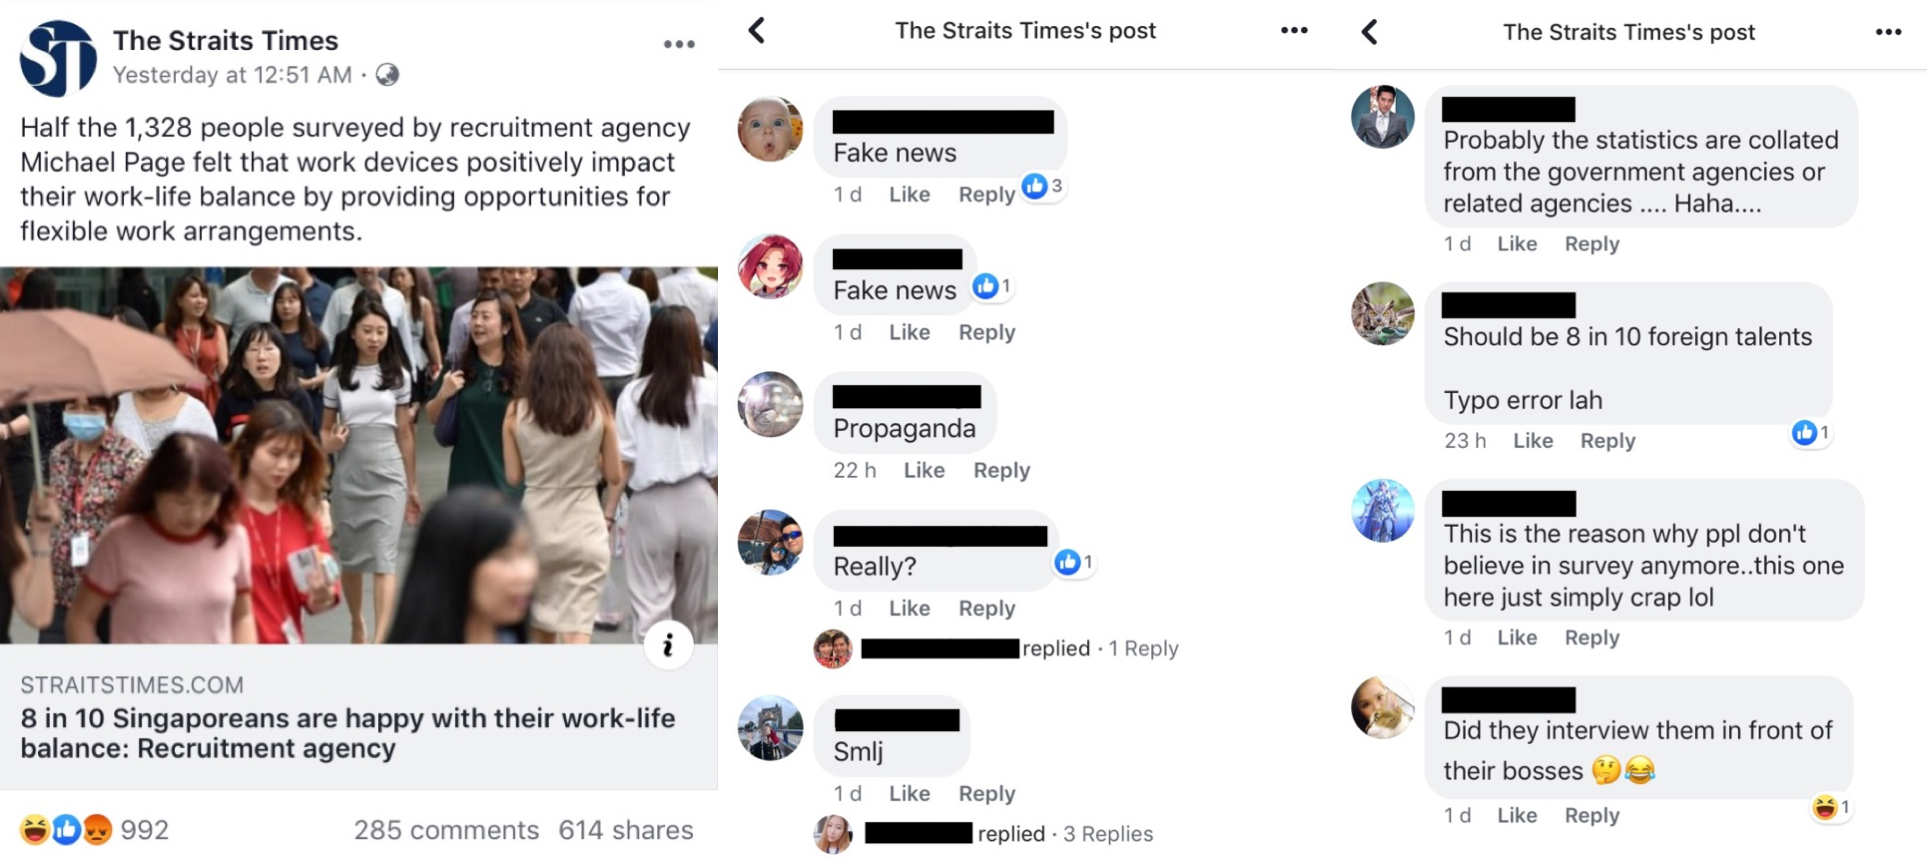
\includegraphics[width=0.9\linewidth]{images/samples/st_worklife} 

}

\caption{Screenshot of online article on work-life balance. Retrieved July 16, 2019.}\label{fig:st-worklife}
\end{figure}

Many people on social media spoke out against the findings (not
unexpectedly), questioning how reliable these findings were. These
commentators probably felt such findings could not possibly reflect
reality, given their own experiences. Surely, they might believe, more
people are unhappy with their work-life balance. To rationalize this
incongruence, there will inadvertently be some attention drawn to the
sample size.

\begin{figure}

{\centering 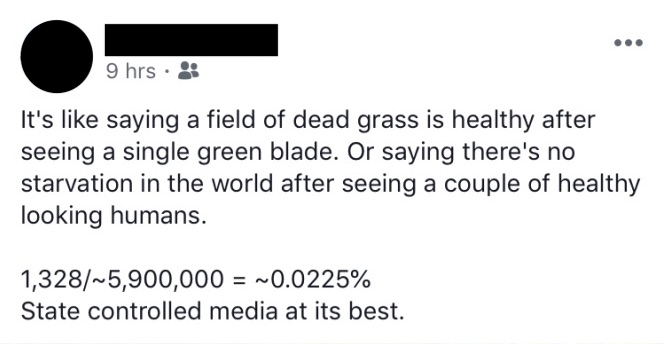
\includegraphics[width=0.6\linewidth]{images/samples/st_samplesize} 

}

\caption{Screenshot of comment on work-life balance article. Retrieved July 16, 2019.}\label{fig:st-samplesize}
\end{figure}

The comment above (Figure \ref{fig:st-samplesize}) shows how people
often rationalize their feelings toward studies that don't reflect their
own perception\footnote{For studies that do agree with the layperson's
  perception, one probable response would be that it is ``common sense''
  and that there is ``no need to do a study to know this''.}. How can
1328 survey respondents represent an entire population of approximately
5.9 million individuals?

The frustrating thing about the
\href{https://www.michaelpage.com.sg/advice/career-advice/work-life-balance/singapore-happy-work}{report
by Michael Page} is that it is \textbf{not transparent about its
methodology}. Without this information, we cannot know for sure about
how generalizable these findings are to the whole population. They
likely cannot say much about \emph{all Singaporeans} - the results may
be limited to Singaporeans who took the survey, who may be a very
different group of Singaporeans compared to those who did not take the
survey.

This is not an isolated case - it often is difficult to find out exactly
how surveys like these (that is, surveys aimed at generating public
interest and reported by the media) were conducted. As we will see, the
key questions are these: \textbf{How were respondents recruited, and how
is uncertainty being estimated?}

\section{Size matters, but how so?}\label{size-matters-but-how-so}

It is true that size matters. However, people tend to paint some variant
of this false dichotomy - results are accurate if the sample size is
arbitrarily large (e.g., \textasciitilde{}50k individuals, or some
percentage of the population size), and completely inaccurate otherwise.
But more data doesn't necessarily mean appropriate data. For instance,
having data on all Singaporean Chinese doesn't really help me understand
Singaporean Malays better. The dichotomy is also terribly unhelpful,
because what we want is to be able to draw big conclusions from small
data\footnote{The obsession with big data is sometimes misguided,
  especially if this suggests `small data' is useless or inferior. Big
  data is mostly useful for other reasons rather than its `bigness'
  (i.e., the sheer number of observations). See Matthew Salganik's
  subsection on this in his book \emph{Bit by Bit} for a good treatment
  of this subject:
  \url{https://www.bitbybitbook.com/en/1st-ed/observing-behavior/characteristics/big/}}.
In fact, we do this all the time - we conduct interviews to hire people,
we date others before entering into a serious relationship, we
administer written tests to measure area-specific knowledge, we audition
actors before casting them in a role, and more. While understanding that
these processes are not perfect, we do expect them to provide us with
sufficient information on which to base our bigger decisions.

\textbf{But how certain can we be?} This question is key. First, we need
the following information: what are the sampling probabilites for each
respondent in the sample? In other words, how likely is each member to
be selected into the sample? If they were selected at random\footnote{Random
  here means that every person in the population has an equal (or known)
  chance of being selected. It does not mean I randomly approach someone
  on the street, since certain types of people are more likely to be
  selected with this method (e.g., people who live close to that street,
  people who are around at that time, etc.). Usually, in Singapore,
  researchers who want a random sample get a list of household addresses
  from the Department of Statistics. It is assumed that the Department
  of Statistics provides a random sample of all household addresses, but
  I am not privy to what happens exactly.}, there are established
methods to calculate uncertainty around our findings\footnote{Via the
  Central Limit Theorem. If the quantity of interest is a
  proportion/probability, then the normal approximation property (and
  its assumptions) also needs to be invoked. The point here, however, is
  not to demonstrate the Central Limit Theorem, but to demonstrate how
  sample size matters. I will therefore avoid getting into the
  technicalities of the Central Limit Theorem.}.

Let's do a small simulation exercise here to demonstrate how these
calculations work, without having to read the math\footnote{If you
  already understand what
  \(\lim_{n \to \infty} \Pr\left[\frac{\sqrt{n}(S_n - \mu)}{\sigma} \leq x \right]= \Phi(x)\)
  means, you may skip ahead to the next section}. Code here is written
in R. A simulation means that we can determine what is the `truth' in a
hypothetical population, and then use the computer to draw samples from
this population\footnote{The code here utilizes the Monte Carlo method,
  which essentially is a computational way to see how samples perform
  under realistic data conditions with a known probability distribution.}
to see how sampling (and sample sizes) work. Our quantity of interest is
the proportion of people who like durian. We define the population such
that 65\% of people (in our population) like durian (i.e.,
\(\Pr(\text{Likes Durian}) = 0.65\))\footnote{Look at Chapter
  \ref{ooptech} for a short explanation of how we went from proportions
  to probabilites}.

\begin{Shaded}
\begin{Highlighting}[]
\CommentTok{# Determine the sample size }
\NormalTok{n <-}\StringTok{ }\DecValTok{100}

\CommentTok{# Draw samples from a population, where Pr(Likes Durian) = 0.65}
\NormalTok{sample <-}\StringTok{ }\KeywordTok{rbinom}\NormalTok{(n, }\DecValTok{1}\NormalTok{, }\DataTypeTok{p=}\FloatTok{0.65}\NormalTok{)}

\CommentTok{# Calculate the proportion of people who report liking durian}
\KeywordTok{sum}\NormalTok{(sample)}\OperatorTok{/}\NormalTok{n}
\end{Highlighting}
\end{Shaded}

\begin{verbatim}
## [1] 0.61
\end{verbatim}

The number produced above is 0.61, but if you run the code above
multiple times, you will realize the number produced is different each
time you run it (i.e., each time you draw a new sample). This makes
sense, since samples are drawn randomly. Since we know the true value of
\(\Pr(\text{Likes Durian})\), we also know how far off these sample
estimates of \(\Pr(\text{Likes Durian})\) tend to be. The next step in
this exercise is to draw a large number of samples of the same size to
show how much these sample proportions can vary.

\begin{Shaded}
\begin{Highlighting}[]
\CommentTok{# Determine the sample size}
\NormalTok{n <-}\StringTok{ }\DecValTok{100}

\CommentTok{# Draw 10000 samples of the same size}
\NormalTok{sample_no <-}\StringTok{ }\DecValTok{1}\OperatorTok{:}\DecValTok{10000}
\NormalTok{samples <-}\StringTok{ }\KeywordTok{lapply}\NormalTok{(sample_no, }\ControlFlowTok{function}\NormalTok{(x) }\KeywordTok{rbinom}\NormalTok{(n,}\DecValTok{1}\NormalTok{,}\DataTypeTok{p=}\FloatTok{0.65}\NormalTok{))}
\NormalTok{proportions <-}\StringTok{ }\KeywordTok{lapply}\NormalTok{(samples, }\ControlFlowTok{function}\NormalTok{(x) }\KeywordTok{sum}\NormalTok{(x)}\OperatorTok{/}\NormalTok{n)}

\CommentTok{# Visualize the proportions with a histogram}
\KeywordTok{hist}\NormalTok{(}\KeywordTok{unlist}\NormalTok{(proportions), }
     \DataTypeTok{main=}\StringTok{"Distribution of Proportions"}\NormalTok{, }
     \DataTypeTok{xlab=}\StringTok{"Proportion"}\NormalTok{)}
\end{Highlighting}
\end{Shaded}

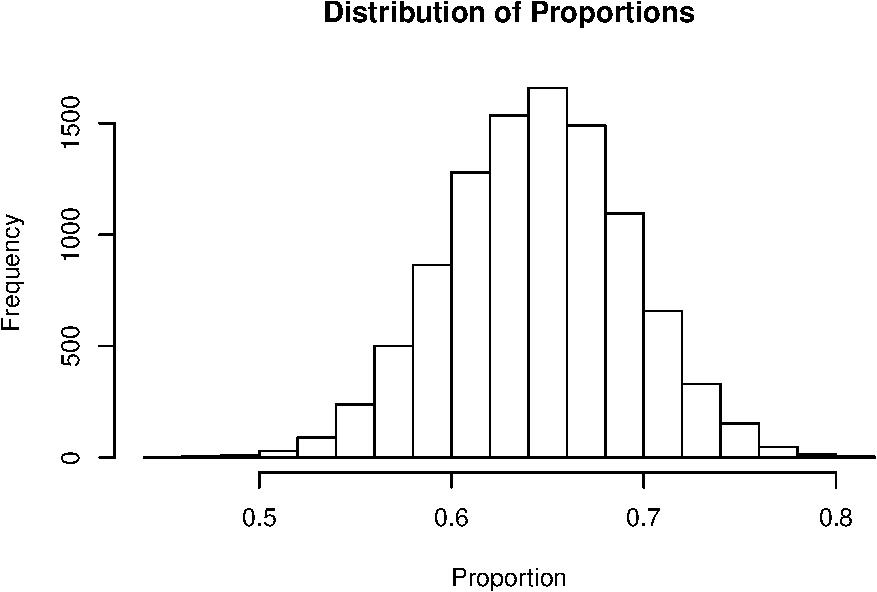
\includegraphics{bookdown_files/figure-latex/unnamed-chunk-11-1.pdf}

You can see that the distribution of proportions from these samples
looks (somewhat) like a bell curve\footnote{Or, in statistics speak, it
  is approximately normally distributed. This will remind you of the
  Central Limit Theorem, if you're familiar.}. Let's now summarize this
distribution with some numbers.

\begin{Shaded}
\begin{Highlighting}[]
\CommentTok{# Get the mean of all proportions, }
\CommentTok{#  rounded to 2 decimal places}
\KeywordTok{round}\NormalTok{(}\KeywordTok{mean}\NormalTok{(}\KeywordTok{unlist}\NormalTok{(proportions)),}\DecValTok{2}\NormalTok{)}
\end{Highlighting}
\end{Shaded}

\begin{verbatim}
## [1] 0.65
\end{verbatim}

\begin{Shaded}
\begin{Highlighting}[]
\CommentTok{# Get the 2.5th and 97.5th percentiles}
\KeywordTok{quantile}\NormalTok{(}\KeywordTok{unlist}\NormalTok{(proportions), }\DataTypeTok{prob=}\KeywordTok{c}\NormalTok{(}\FloatTok{0.025}\NormalTok{, }\FloatTok{0.975}\NormalTok{))}
\end{Highlighting}
\end{Shaded}

\begin{verbatim}
##  2.5% 97.5% 
##  0.56  0.74
\end{verbatim}

\textbf{What do these numbers tell us?} If you realize, the mean of the
distribution of sample proportions is, in fact, the true value of
\(\Pr(\text{Likes Durian})\). This demonstrates that even with
relatively small samples, it is possible to recover the true population
value through repeated sampling. The only difficulty is that we can
seldom get so many samples, so the quantile values are of more help. The
quantile values tell us that 95\% of all the sample proportions will
fall between 0.57 and 0.74. This gives us some measure of uncertainty.
In other words - if I take a single sample of size 100, 95\% of the time
the proportion of those who like durian calculated from this sample will
fall between 0.57 and 0.74 (given that the true value is 0.65)\footnote{Other
  than the sample size, uncertainty also increases if the true value of
  \(\Pr(\text{Likes Durian})\) is closer to 0.50.}. In other words, for
this particular scenario (i.e., 100 observations, true proportion =
0.65), sample estimates will differ from the true value by at most 9
percentage points 95\% of the time. This is the fundamental basis of
claims by researchers that a survey has a certain ``margin of error''.

\textbf{So what happens when we increase the sample size?} Let us run
the same code again, but increase the sample size to 1000.

\begin{Shaded}
\begin{Highlighting}[]
\CommentTok{# Determine the sample size}
\NormalTok{n <-}\StringTok{ }\DecValTok{1000}

\CommentTok{# Draw 10000 samples of the same size}
\NormalTok{sample_no <-}\StringTok{ }\DecValTok{1}\OperatorTok{:}\DecValTok{10000}
\NormalTok{samples <-}\StringTok{ }\KeywordTok{lapply}\NormalTok{(sample_no, }\ControlFlowTok{function}\NormalTok{(x) }\KeywordTok{rbinom}\NormalTok{(n,}\DecValTok{1}\NormalTok{,}\DataTypeTok{p=}\FloatTok{0.65}\NormalTok{))}
\NormalTok{proportions <-}\StringTok{ }\KeywordTok{lapply}\NormalTok{(samples, }\ControlFlowTok{function}\NormalTok{(x) }\KeywordTok{sum}\NormalTok{(x)}\OperatorTok{/}\NormalTok{n)}

\CommentTok{# Get the 2.5th and 97.5th percentiles}
\KeywordTok{quantile}\NormalTok{(}\KeywordTok{unlist}\NormalTok{(proportions), }\DataTypeTok{prob=}\KeywordTok{c}\NormalTok{(}\FloatTok{0.025}\NormalTok{, }\FloatTok{0.975}\NormalTok{))}
\end{Highlighting}
\end{Shaded}

\begin{verbatim}
##  2.5% 97.5% 
## 0.620 0.679
\end{verbatim}

You will realize here that the interval for the quantile values have
narrowed\footnote{If you calculate the mean of proportions again, you
  will also realize also that it recovers the true value of 0.65}. This
shows that with a bigger sample size, our uncertainty around the true
estimate also shrinks.

Our little simulation exercise has shown a number of things:

\begin{enumerate}
\def\labelenumi{\arabic{enumi}.}
\tightlist
\item
  The basic intuition is correct - larger sample sizes in fact produce
  estimates that are less susceptible to sampling error (that is,
  estimates generally fall closer to the true value).
\item
  However, this basic intuition matters less than we often think. Even a
  relatively small sample size of 1000 (as asserted by the commentator
  in Chapter \ref{sample-worklife}) produces estimates quite close to
  the true value (in this case, within 3 percentage points 95\% of the
  time).
\end{enumerate}

What is important here, however, is that these estimates can only be
calculated in this manner if we have a probability sample - that is, if
we know the sampling probabilites for each respondent in the
sample\footnote{The easiest way is to get a simple random sample (where
  everyone has an equal chance of selection), but there are also ways to
  adjust for more complex cases (e.g., multistage sampling)}. \textbf{If
we do not know how respondents in a sample were recruited, there is no
way to determine whether purported findings actually reflect the
population, and how much uncertainty there is around them}.

This is not to say that there is no way to calculate a ``margin of
error'' or bounds of uncertainty for non-probability samples.
Researchers have been developing new and innovative ways to recover
reliable estimates even with non-probability samples, as ``big data''
comes to the forefront. Unfortunately, people are often careless and
apply methods meant for probability samples to non-probability samples,
expecting them to work in the same way. We will explore this in the next
section.

\section{Non-probability sample, now
what}\label{non-probability-sample-now-what}

Probability samples are hard to come by, and while in theory they are
the ``gold standard''\footnote{Apart from having information on the
  entire population, through a census or administrative government data.},
there are a number of drawbacks when trying to implement them:

\begin{enumerate}
\def\labelenumi{\arabic{enumi}.}
\tightlist
\item
  Poor response rates. Not all respondents in your probability sample
  will agree to respond to your survey or participate in your study.
  While researchers have tried various methods (e.g., offering a
  monetary ``token of appreciation'') to increase response rates, low
  response rates threaten the validity of a probability sample,
  especially if those who refuse are systematically different from those
  who eventually participate.
\item
  High cost. Partly because of strategies to increase response rates
  through ``tokens of appreciation'', the cost of implementing a
  high-quality survey (especially through traditional face-to-face
  interviews) with a probability sample have increased substantially.
\end{enumerate}

Some researchers, therefore, have turned to online surveys (which are
much cheaper to conduct).
\href{https://lkyspp.nus.edu.sg/docs/default-source/gia-documents/cars_-condos-and-cai-png-survey-(high-res).pdf}{One
recent study commissioned by the Lee Kuan Yew School of Public Policy}
on Singaporeans' perception of class markers did this.

\begin{figure}

{\centering 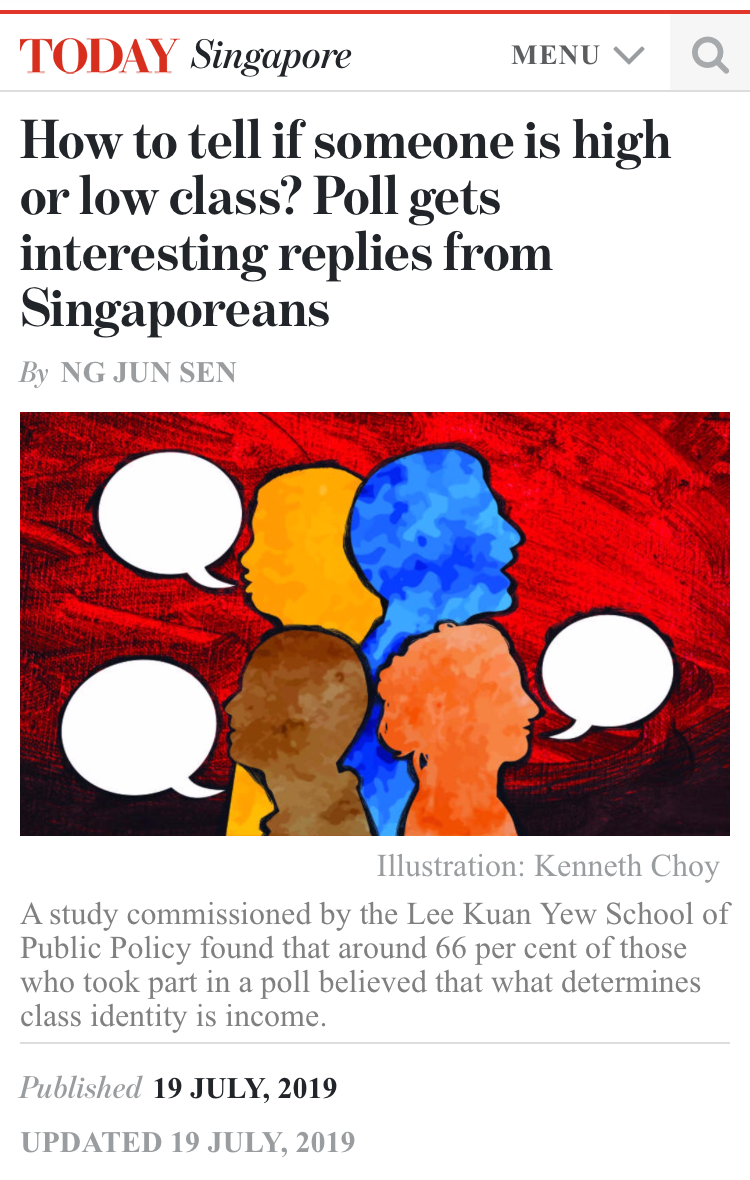
\includegraphics[width=0.5\linewidth]{images/samples/today_classpercept} 

}

\caption{Screenshot of TODAYonline article on class perceptions. Retrieved July 16, 2019.}\label{fig:today-classmarkers}
\end{figure}

The newspaper article reports the following:

\begin{quote}
While Dr Dodgson acknowledged that the sample size was relatively low,
with a 4.25 per cent margin of error, she told TODAY that the open-ended
nature of the survey ``gave greater nuance and accuracy'' than
multiple-choice questionnaires.
\end{quote}

\href{https://lkyspp.nus.edu.sg/docs/default-source/gia-documents/cars_-condos-and-cai-png-survey-(high-res).pdf}{The
study report} also contains the following `infographic', which confirms
what the news article reported.

\begin{figure}

{\centering 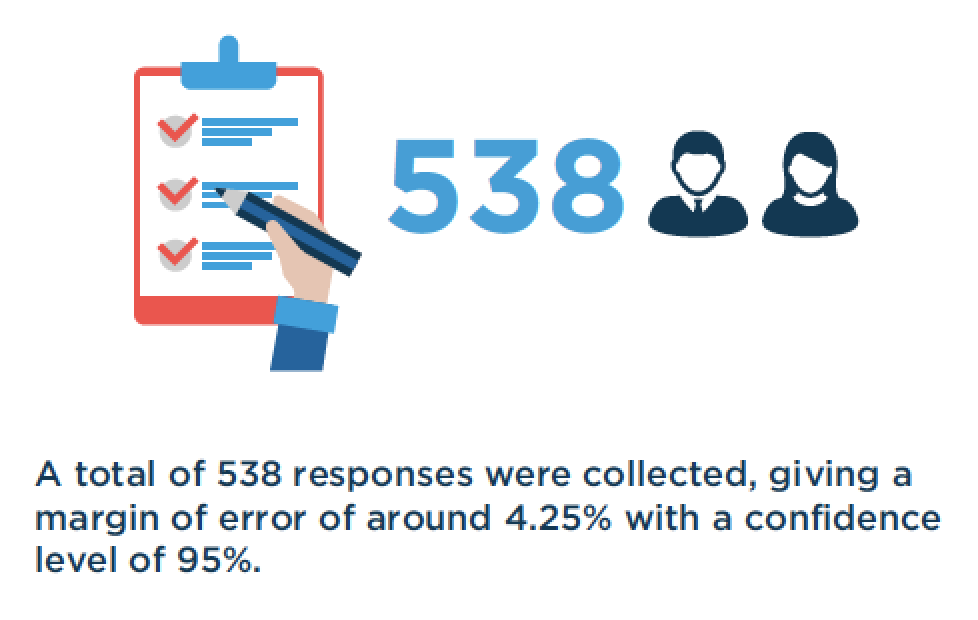
\includegraphics[width=0.6\linewidth]{images/samples/lkyspp_reportsample} 

}

\caption{Screenshot of TODAYonline article on class perceptions. Retrieved July 16, 2019.}\label{fig:today-reportsample}
\end{figure}

As you may recognize, this ``margin of error'' is something we had
talked about in the previous section. I simulated the results to show
the basic reasoning behind sampling theory, but you can in fact easily
find online calculators purporting to calculate this ``margin of error''
for you\footnote{These calculators use closed-form formulas to produce a
  `margin of error', rather than through the more
  numerical/computational approach I used.}. Let's use a
\href{http://www.raosoft.com/samplesize.html}{random one I found}. Just
change the margin of error to 4.25 and the population size to
\textasciitilde{}3.5 million (Singapore resident population size) and
you get back a recommended sample size of \textasciitilde{}530\footnote{The
  report itself does not state how they calculated the margin of error.
  It is my guess that this (or a variant of this calculation) is what
  they did. If you are aware that a different method was used, please
  write to me so I can correct it.}. But remember, \textbf{these
calculations are for a probability sample!}\footnote{More specifically,
  a simple random sample.}

Is the study in question conducted with a probability sample? The
details provided are rather vague\footnote{For instance, how did the
  panel responses service recruit participants?}, but my general sense
is that they were not using a probability sample. The report states
that:

\begin{quote}
Responses were solicited via social media and via a panel responses
service. The goal with this was to attract a mixture of opinions, both
from people with a pre-existing interest in the topic (whose opinions
are generally weighted more heavily in political discussion, simply
because they are more likely to assert them and eventually to take
action on the same basis) and from those with no immediate interest
(whose opinions are often discounted in political discussion, but which
can have startling effects at the ballot box). Similarly, the
demographics of the respondents were tracked with the aim of creating a
sample that would be broadly representative of the general population.
\end{quote}

In what seems like implicit acknowledgement that the study did not use a
probability sample, some effort has been made to ensure adequate
`representation' through varied modes (social media and panel responses
service), and through mimicking the country's demographic composition
(probably by ensuring sufficient numbers of minorities)\footnote{This
  appears similar to quota sampling, which is a non-probability sampling
  method.}. It is worth noting, however, that in no way does this make
it equivalent to a probability sample of \emph{all
Singaporeans}\footnote{If only it were that simple.}. \textbf{It is
therefore inappropriate to calculate and use a margin of error \emph{as
if} it were a probability sample of all Singaporeans.}

This does not mean that there is no way to use a non-probability sample
to produce accurate estimates. But methods to derive estimates from
non-probability samples are often context dependent (i.e., they have to
be customized for each case, depending on the quantity of interest) and
have different requirements beyond sample size. It requires more effort
from researchers, but this is not necessarily a bad thing. Because of
the practical drawbacks of probability sampling (highlighted above),
statistical innovation to draw inferences from non-probability samples
(often done through post-sampling adjustments) is much needed in the
world of research.

`Big data' plays an important role here. (Matthew Salganik gives one of
the best overviews on the characteristics of `big data'
\href{https://www.bitbybitbook.com/en/1st-ed/observing-behavior/characteristics/}{in
his book \emph{Bit by Bit}}, which I highly recommend). Data that is
collected constantly and from many people at once allows for timely and
cost-effective results, if we use the right approach to analyze them.
\citet{wang_forecasting_2015} (available
\href{http://www.stat.columbia.edu/~gelman/research/published/forecasting-with-nonrepresentative-polls.pdf}{here})
use multilevel regression and poststratification (affectionately called
``Mister P'') to show that accurate forecasts of the 2012 US
presidential election could be obtained using data from Xbox\footnote{A
  gaming platform} users. Two points are of note here. First, the sample
was large - 750,148 interviews were conducted through Xbox polls, with
345,858 unique respondents, and over 30,000 respondents completed five
or more polls. Second, having strong covariates\footnote{Other
  characteristics of the sample, beyond basic demographic information.}
to adjust for non-response bias (\citet{gelman_mythical_2016}, available
\href{http://www.stat.columbia.edu/~gelman/research/published/swingers.pdf}{here})
and subgroup level characteristics (if more granular subgroup level
estimates are of interest) are crucial to good estimation\footnote{See
  also
  \url{https://statmodeling.stat.columbia.edu/2013/10/09/mister-p-whats-its-secret-sauce/}}.
\textbf{Neither of these was true in the study by the Lee Kuan Yew
School of Public Policy discussed above.} Of course, this does not mean
\emph{all} of the claims in that study are invalid. There are probably
still insights worth learning from. However, it does tell us that we
need to constantly evaluate the claims of studies against their
methodology - understanding the \emph{how} is often key.

\section{Conclusion}\label{conclusion-2}

We have discussed sampling - what probability samples and
non-probability samples are. It is true that sample size matters, but we
can quantify the uncertainty in smaller samples by calculating
bounds/intervals around our estimates. This is quite simple to do if we
have a probability sample, and in such cases, estimates are quite
accurate even with a relatively small sample size (e.g., 1000
observations).

In many studies reported in the media, however, non-probability samples
are used. Non-probability samples can be a good alternative to
probability samples especially given that non-response rates are
increasing. \textbf{However, we cannot use formulas meant for
probability samples and apply them to non-probability samples as if they
are the same.} Non-probability samples require different (and slighty
more complex) methods to produce equally accurate estimates.

What does this case study highlight? First, we need to be
transparent\footnote{And we need to demand transparency.} about how
studies recruit members into their sample. \textbf{How the sample is
recruited is usually much more important than how large the sample is},
but we are seldom given enough detail about it. Second, we need to be
aware if appropriate methods are being used. Using a non-probability
sample can seem more practical, but we become overconfident and may end
up with the wrong conclusions if we simply act as if it is a probability
sample.

\chapter{What kind of societal change?}\label{apc}

\begin{verbatim}
Contributor: Shannon Ang
Date: 17 September 2019
\end{verbatim}

We hear various statistics that imply social change all the time. For
instance, we hear that
\href{https://www.channelnewsasia.com/news/singapore/suicides-number-2018-teenagers-boys-highest-11761480}{suicides
are rising in Singapore}, or that
\href{https://www.todayonline.com/singapore/singaporeans-living-longer-spending-greater-proportion-time-ill-health-study}{Singaporeans
are living longer}, or that the
\href{https://www.channelnewsasia.com/news/singapore/number-of-babies-born-in-singapore-falls-to-lowest-in-8-years-11743722}{number
of babies born is declining}.

As always, people have many comments and theories about reasons behind
what is happening. But before we can evaluate these comments, we need to
first understand - what do these numbers really mean, and what kind of
change is it really capturing? This case study looks at several ways we
talk about societal change in public, and provides a better
understanding of these commonly used numbers for higher quality
discourse.

\section{Three ways to understand
change}\label{three-ways-to-understand-change}

Before we go evaluate real examples, it will be helpful to understand
different kinds of societal change. Let us work with a toy example.
Suppose the newspaper (your favourite one) headline tomorrow states:
``Average walking speed of Singaporeans slower than 10 years ago''.
There are three possible explanations for this (maybe more, this is not
a perfect analogy).

\begin{enumerate}
\def\labelenumi{\arabic{enumi}.}
\item
  Older people walk slower, and Singapore is an ageing society (average
  age is rising), so its average walking speed will fall as there are
  more older people in society.
\item
  Those born later (e.g., Millenials, Gen Z) are walking slower than
  those born earlier (e.g., Baby Boomers), bringing down our average
  walking speed.
\item
  There was an alien invasion this year and many aliens suddenly came to
  live among us. This suddenly caused overpopulation, since our system
  \href{https://www.strategygroup.gov.sg/media-centre/population-white-paper-a-sustainable-population-for-a-dynamic-singapore}{is
  only prepared for 6.9 million}. People in Singapore thus have to lower
  their walking speed this year because it has become very crowded
  compared to last year.
\end{enumerate}

The last one is slightly facetious, but as you can see, the three
explanations point to three \textbf{quite different} reasons for change.
We will look at each one, in order.

\begin{enumerate}
\def\labelenumi{\arabic{enumi}.}
\item
  Change with \textbf{age}: Age effects refer to changes over the life
  course that apply to all individuals as they grow older. This is best
  demonstrated in terms of physical and biological changes that occur as
  we age (e.g., our metabolism slows down, we get wrinkles etc.) - such
  changes tend to be common to all of us, regardless of when we were
  born, or what era we live in.
\item
  Change with \textbf{cohort}: Cohort effects are probably easiest to
  think about as \emph{generational} change (i.e., change with
  \emph{birth} cohorts), even though more generally they are used refer
  to a group of individuals that have gone through shared experiences
  (e.g., school cohorts). When you hear remarks like ``\emph{young
  people nowadays} are {[}such strawberries / so spoilt / have no
  manners{]}'', this is usually the kind of change people they are
  suggesting has happened.
\item
  Change with \textbf{period}: Period effects are changes due to
  contextual factors that affect all living persons at a particular
  point in time. For instance, significant events such as wars,
  epidemics, or natural disasters affect everyone who is exposed to it
  regardless of age.
\end{enumerate}

Social scientists have long recognized the need to think clearly about
these three distinct ways of understanding social change\footnote{Although
  there is an equally long-running debate about how to estimate these
  effects, given linear dependence between the terms, i.e.
  \(Cohort = Period - Age\). See \citet{fosse_analyzing_2019} for a
  great discussion.}. Popular discourse, however, tends to ignore the
meaningful differences between these concepts - a common error is making
conclusions about cohort change based off period data. We will examine
two instances of this.

\section{Declines in marriage and divorce}\label{marriage-decline}

Marriage has been a key preoccupation of Singapore society for many
reasons (e.g., getting housing, increasing fertility rates). Trends in
marriage/divorce/fertility are thus often closely watched. The Straits
Times recently published this article on marriage/divorce rates in 2018.

\begin{figure}

{\centering 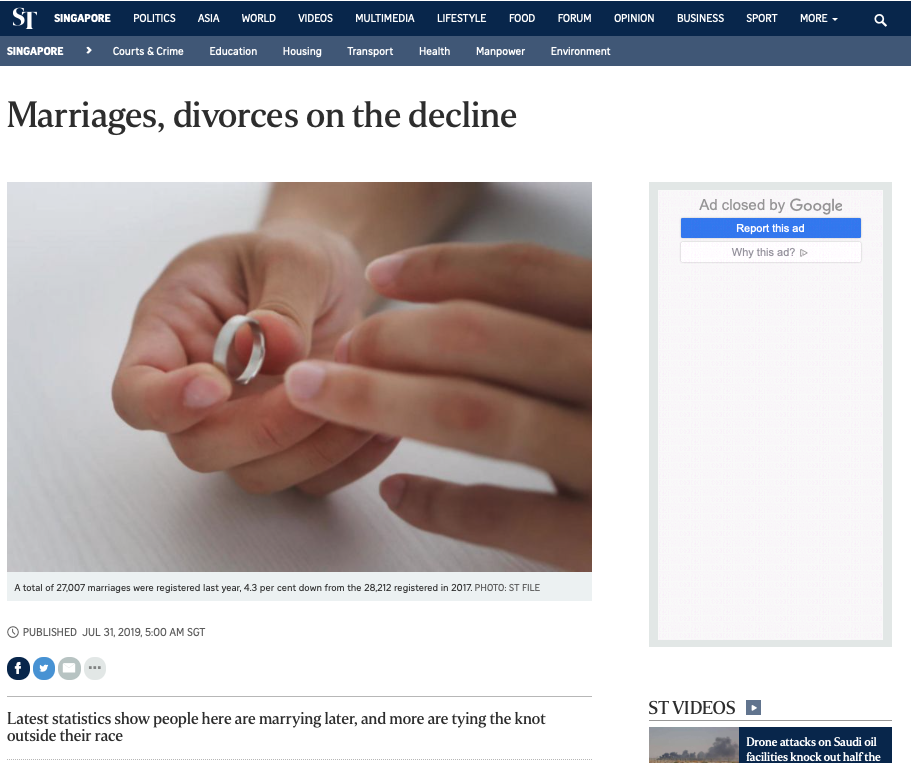
\includegraphics[width=0.8\linewidth]{images/apc/apc_marriage} 

}

\caption{Screenshot of online article on marriage rates. Retrieved September 17, 2019.}\label{fig:st-apcmarriage}
\end{figure}

The article is based on
\href{https://www.singstat.gov.sg/-/media/files/publications/population/smd2018.pdf}{a
report} on Marriages and Divorces, produced by the Department of
Statistics\footnote{We will focus on discussing non-Muslim marriages
  here, but the same principles can be applied to Muslim marriages as
  well.}. Among other things, the article states that:

\begin{quote}
A total of 27,007 marriages were registered last year - the lowest in
five years and 4.3 per cent fewer than the 28,212 marriages registered
in 2017.

\ldots{} Meanwhile, 7,344 marriages ended in a divorce or annulment last
year, a 3.1 per cent drop from the 7,578 marital dissolutions in 2017.

\ldots{} Given the volatile economy, observers said financial
considerations could have contributed to the falling number of marriages
and divorces last year.
\end{quote}

Now, given that we've talked about age, cohort, and period changes, one
question that should come to mind is: \emph{what kind of measure is
this?} Quite obviously, this is a period measure - it records the number
of marriages in a certain year. Unnamed `observers' cited by the article
seem to understand this. They point out that the economy last year may
have had a part to play, which is a plausible reason for period changes
that suits the nature of the measure\footnote{The general marriage rate,
  which is adjusted for population size of unmarried residents aged
  15-49, also seems to tell this story.}. We then move on to the
following paragraph on changes in median age at first marriage:

\begin{quote}
The median age at first marriage for grooms rose from 29.8 years in 2008
to 30.2 years last year, while for brides, it went up from 27.3 years in
2008 to 28.5 years last year.

This is because more people spend a longer time getting an education and
building up their careers before they settle down, said National
University of Singapore sociologist Tan Ern Ser.
\end{quote}

Note here that median age at marriage is also a \emph{period measure} -
of all people who got married that year, half of them got married before
age 28.5. NUS sociologist Tan Ern Ser says that the median age at first
marriage is rising because ``people'' spend more time in education and
early-career building before they ``settle down'' (i.e., get married).
Who are these ``people'', exactly? Since most members of older cohorts
do not usually go back into education and early-career building, there
seems to be an implicit reference to younger cohorts (or, in layman
terms, \emph{``people nowadays''})\footnote{Of course, there is now a
  great drive towards lifelong learning and mid-career switches, but in
  the context I think it is reasonable to assume this is not the group
  of people being referred to.}.

\textbf{How reasonable is it to adopt \emph{cohort} explanations for
changes in \emph{period} measures of marriage?} Frustratingly, marriage
statistics by cohort are not available from the government. The reason
why period measures are used is often a matter of practicality (as we
will discuss in the next section), but in other countries, academics use
longitudinal panel survey data to estimate and project what might happen
in younger cohorts. In Singapore, such survey data is scant and/or tend
not to be shared with researchers outside of the government. This makes
cohort change especially difficult to study.

But we will work with what we have. For a start, let us try to address
one possible concern - that changes in period measures are due to the
changing population age structure. Age-specific marriage rates are
adjusted for the size of age groups, and therefore may be helpful here.
Let's look back to
\href{https://www.singstat.gov.sg/-/media/files/publications/population/smd2018.pdf}{the
report} on Marriages and Divorces by the Department of Statistics, where
we find the figure below.

\begin{figure}

{\centering 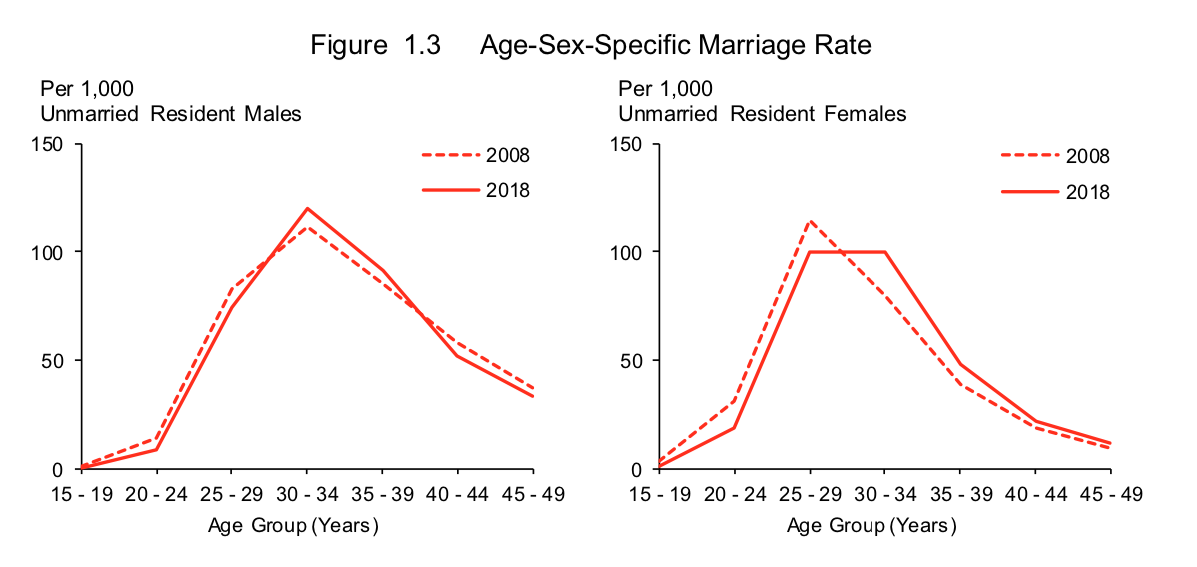
\includegraphics[width=0.8\linewidth]{images/apc/report_fig} 

}

\caption{Screenshot from Department of Statistics report titled "Statistics on Marriages and Divorces,  2018". Retrieved September 17, 2019.}\label{fig:apc-reportsingstat}
\end{figure}

As highlighted by the report, it does seem like people are getting
married at later ages (generally, you can see that the mountain-like
shape in the figure is moving to the right). While we don't have cohort
measures, maybe looking at a mix of period-based and age-based measures
provides us some indication as to whether the cohort explanation being
offered remains a plausible one\footnote{These are not enough, however,
  to confirm what kind of cohort changes have been occuring.}? Perhaps
younger cohorts \emph{are} delaying marriage in view of education and
career building. But even using a mix of period-based and age-based
measures to infer cohort change might be misleading, as we will see
shortly.

Let us now move on to another comment that was made. The news article
states:

\begin{quote}
\ldots{}Singapore Management University professor of sociology
(practice) Paulin Straughan said they also seem to be spending a longer
time looking for the right partner. She said: ``People believe that
marriage is forever and unless they are very sure they have found a life
partner, they wouldn't marry.''
\end{quote}

SMU Professor (Practice) Paulin Straughan surmises that median age at
first marriage is rising because ``people'' wait to be very sure of
their partner. While there may be some kernel of truth here (although no
data is provided to support her point), it is quite unclear what she
really means by this. Is she saying that everyone is delaying marriage
because Singaporean culture has changed over time and people across all
generations are now more careful about who to marry compared to the
past\footnote{Think about what this really means though. How possible is
  it to observe this?} (i.e., a period effect)? Or is she saying that
younger cohorts are now more careful about who to marry\footnote{For
  those more technically oriented, \citet{martin_comment:_2009} has an
  intriguing discussion about age*period interactions masquerading as
  cohort effects.} (i.e.~a cohort effect)?

Regardless of what you think it may be, a natural follow-up question
would be - does this also explain the reason why divorce rates are
falling? If the `waiting to be very sure' explanation holds weight, it
should follow that since people have become more careful to marry,
marriages are probably less likely to end up in divorce\footnote{It
  could also be that \emph{even though} people are more careful, they
  still make choices that end up in divorce, but this is somewhat an
  awkward assumption to make given a plain reading of the comment.}.
People ``waiting longer'' would then be a simple explanation for both
falling marriage and divorce rates! Suppose we adopt this explanation
for falling divorce rates.

Remember, once again, that the divorce numbers mentioned in the news
article are a \textbf{period} measure\footnote{You may also ask, since
  we're dealing with absolute numbers, isn't it obvious that if there
  are less marriages, then there would be less divorces too? This is why
  absolute numbers are seldom helpful when examining societal change. At
  a minimum, we should attempt to look for rates that are adjusted for
  the size of the group at risk.}. Once again, we look at age-specific
rates to determine if the explanation is plausible.

\begin{figure}

{\centering 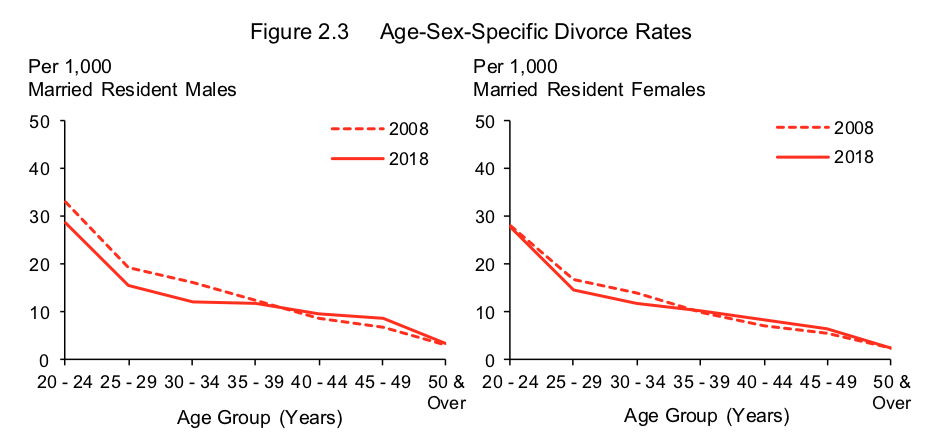
\includegraphics[width=0.8\linewidth]{images/apc/report_fig3} 

}

\caption{Screenshot from Department of Statistics report titled "Statistics on Marriages and Divorces,  2018". Retrieved September 17, 2019.}\label{fig:apc-reportsingstat2nd}
\end{figure}

Indeed, it seems like people are getting divorced at older ages compared
to 2008. Divorce numbers thus do not seem to be driven by changes in
population age composition. This is the same situation as before (with
marriage numbers) - perhaps we can use a mix of period-based and
age-based measures to support a cohort interpretation. But how well does
this explanation really cohere with true \emph{cohort} trends?

Data on divorce trends by birth cohort are, once again, not available
from the government. Weirdly enough, however, there seems to be some
information on divorce by ``marriage cohorts'' (where each cohort is
defined by the year they got married - i.e., if you got married in the
same year as I did, you are in my marriage cohort) in a report by the
Ministry of Social and Family Development (found
\href{https://www.msf.gov.sg/research-and-data/Research-and-Data-Series/Pages/default.aspx}{here}).
What kind of change marriage cohort trends really capture is quite hard
to say, but for heuristic purposes we will assume they roughly
approximate\footnote{Think about who gets married in a certain year.
  What kind of people are they composed of? What characteristics do they
  share? It is hard to say. Other than sharing the same year of
  marriage, diversity within marriage cohorts is likely to be huge. We
  can only assume that younger birth cohorts will dominate most of the
  marriages in later years, but it remains to be seen whether this is
  accurate.} birth cohort trends. The graph below shows us the
proportion of divorces (y-axis) that happen before the couples'
\(x^{th}\) anniversary (shown on the x-axis), by marriage cohort
(indicated by the color and shape of the lines).

\begin{figure}

{\centering 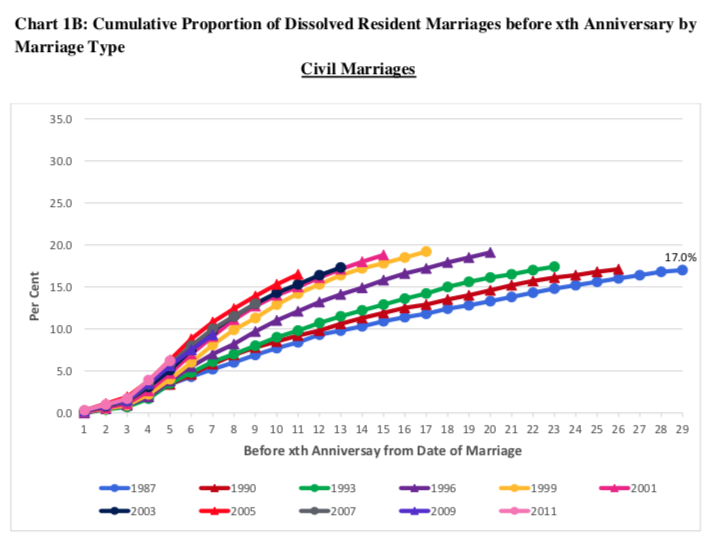
\includegraphics[width=0.8\linewidth]{images/apc/report_fig2} 

}

\caption{Screenshot from Ministry of Social and Family Developent report titled "Dissolutions of Marriages Among Marriage Cohorts, 1987-2015". Retrieved September 17, 2019.}\label{fig:apc-reportmsf}
\end{figure}

What can be observed here is that \textbf{younger (marriage) cohorts
seem to be getting divorced earlier}\footnote{It remains to be seen if
  lifetime divorce rates will be higher, since we cannot yet observe the
  full trajectory of union dissolutions for the younger cohorts (or even
  for older cohorts, since not all of them have disolved their union or
  passed away).}. For instance, you may notice that a higher proportion
of those married in 2011 (light pink line) dissolve their unions before
their 5th anniversary compared to those married in 2001 (dark pink line)
or earlier\footnote{Note that this does not really line up with the 2018
  and 2008 measures we were comparing before, but there really is no
  easy way to do this.}. The picture painted here seems more
bleak\footnote{Assuming divorce is always a bad thing, which may not
  always be the case. A rise in divorce rates may possibly reflect
  changes in power dynamics within couples, with women becoming more
  independent and more willing to leave abusive situations.} compared to
what we expected from period trends (and the news article), which
suggested that divorce rates were falling\footnote{Note that the
  Department of Statistics
  \href{https://www.singstat.gov.sg/-/media/files/publications/population/smd2018.pdf}{report}
  also has age-specific divorce rates, which seems to tell a similar
  story as the period trends - that divorce rates are falling among
  those who are younger (but rising at older ages). This may however
  simply be a function of delayed marriages in general leading to
  delayed divorces}, or that marriages were becoming more stable as a
result of more careful partner selection.

This suggests that \textbf{while period measures and cohort measures can
sometimes tell similar stories about societal change, there are many
times when they do not.} When we say ``marriages and divorces are
falling'', we need to be clear what the data allows us to say, and what
kinds of explanation we give. In the next section, we will look at life
expectancy - a highly misunderstood measure in popular discourse.

\section{Living longer than you
expect}\label{living-longer-than-you-expect}

We've heard this so many times - ``life expectancy is increasing''.
``Singapore has one of the highest life expectancies in the world.''
\textbf{But what does the term ``life expectancy'' mean?}

\begin{figure}

{\centering 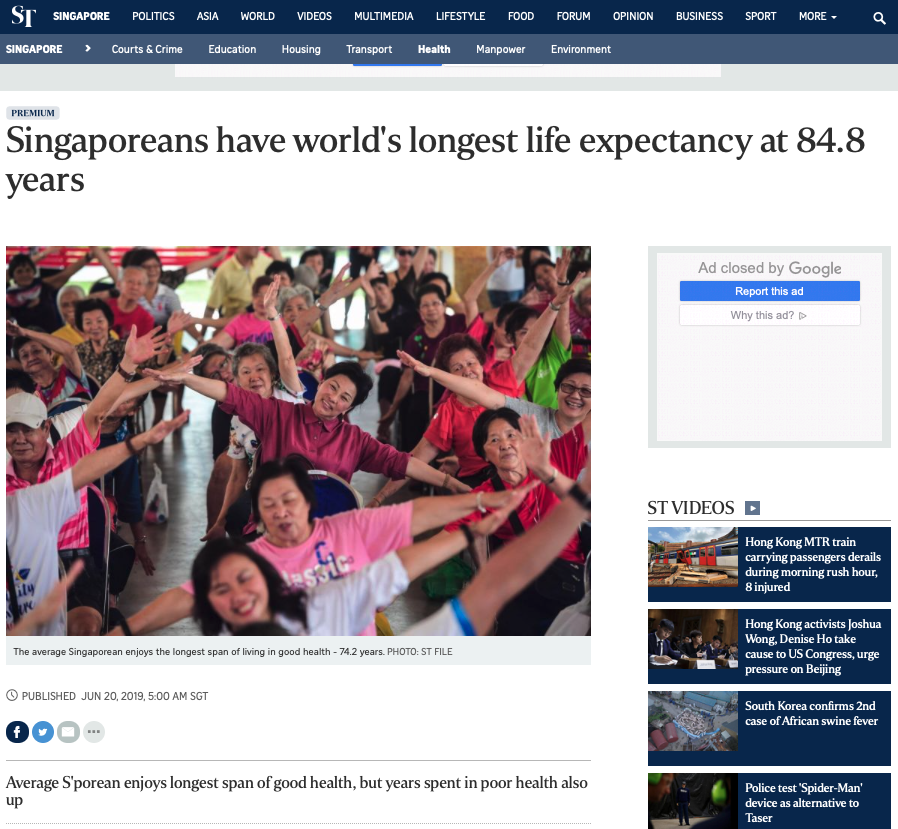
\includegraphics[width=0.8\linewidth]{images/apc/apc_lifeexpectancy} 

}

\caption{Screenshot of online article on life expectancy. Retrieved September 17, 2019.}\label{fig:apc-lifeexp}
\end{figure}

A typical article (such as
\href{https://www.healthxchange.sg/seniors/healthy-ageing/why-singaporeans-living-longer}{this
one} written by a physician) will use estimates of life expectancy to
say, for instance, ``Singaporean residents can expect to live up to 83.2
years (\emph{the figure for 2017})''. This reading of life expectancy is
quite common.

The obvious question here is - Who can expect to live up to 83.2 years?
My grandma? Me? My child? Do all Singaporeans now expect to live to the
same age\footnote{If this is true, then if life expectancy increases
  faster than one year annually, does this mean we can all expect to be
  immortal? You can see how ludicrous this sounds.}?

The figure most often cited in the media is life expectancy \emph{at
birth}. A more precise way to interpret the life expectancy in 2017 is
``Singaporean residents \textbf{who are born in 2017} can expect to live
to 83.2''.
\href{https://www.straitstimes.com/singapore/health/singapore-tops-in-life-expectancy-at-848-years}{This
other news article in the Straits Times} rightly refers to the life
expectancy estimate as ``expected lifespan at birth''.

But this still does not fully capture how life expectancy is calculated.
To do this, we need to go back to our understanding of age, period, and
cohort measures. Life expectancy, as it is reported yearly, is a
\textbf{period measure}.

Without going into full detail (interested readers can refer to
resources such as
\href{https://www.measureevaluation.org/resources/training/online-courses-and-resources/non-certificate-courses-and-mini-tutorials/multiple-decrement-life-tables/lesson-3}{this}),
I will explain briefly how this is calculated. A typical life table from
the Department of Statistics (taken from
\href{https://www.singstat.gov.sg/-/media/files/publications/population/lifetable17-18.pdf}{this
report}) looks like this (this is just the top part, the entire table is
a few pages long):

\begin{figure}

{\centering 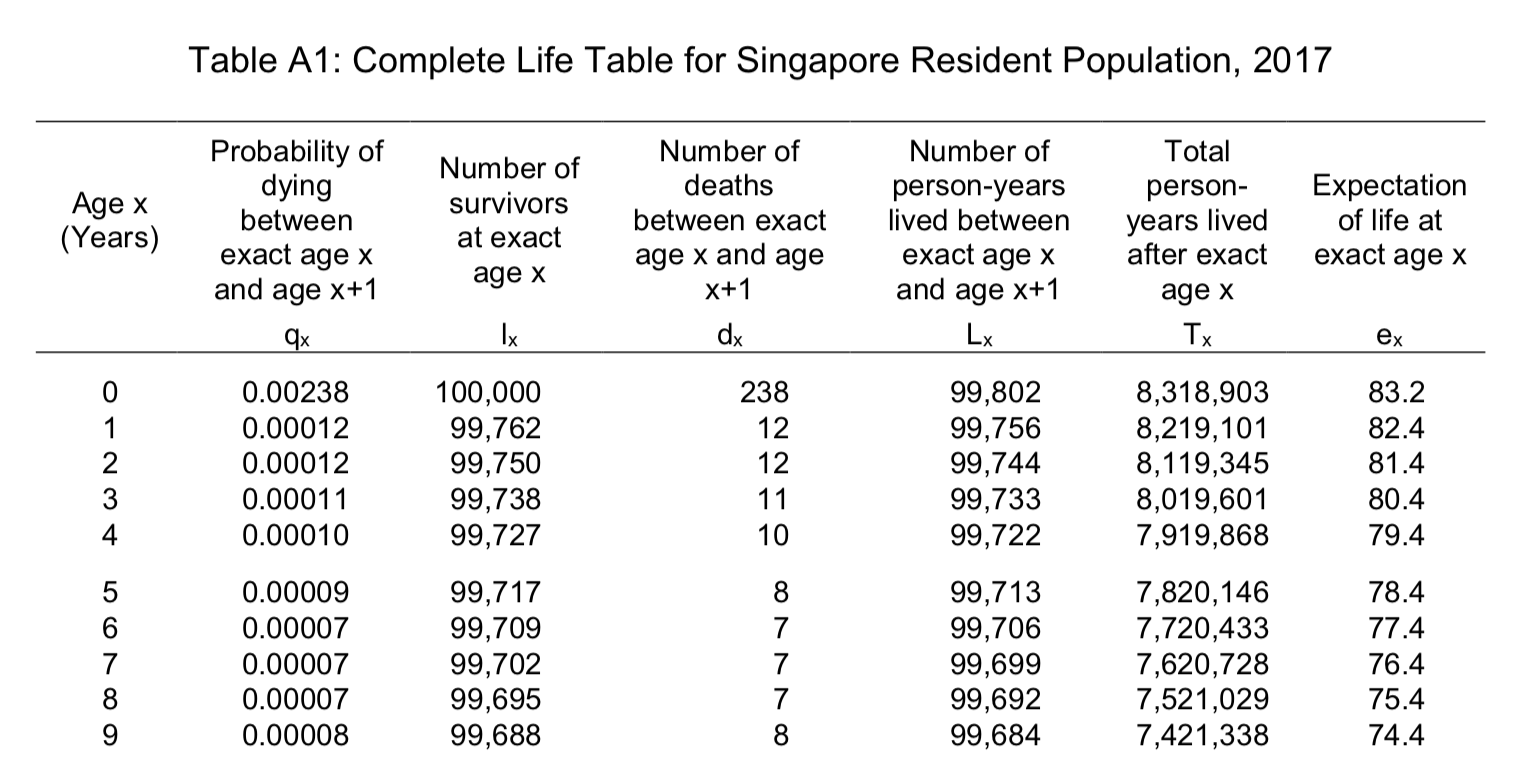
\includegraphics[width=0.8\linewidth]{images/apc/apc_lifetable} 

}

\caption{Screenshot of Complete Life Table from the Department of Statistics. Retrieved September 17, 2019.}\label{fig:apc-lifetable}
\end{figure}

\begin{enumerate}
\def\labelenumi{\arabic{enumi}.}
\item
  Age-specific mortality rates (not pictured, but often referred to as
  \(m_x\)) for a specific year are obtained from the national mortality
  database and turned into\footnote{Some assumptions need to be made
    here about a quantity called \(a_x\), which captures when most
    deaths in a certain age-interval happen within the time period, but
    usually this calculation is straightforward.} the probability of
  dying in a specific age-interval (\(q_x\), pictured).
\item
  You start with a hypothetical base population, usually 100,000, and
  you put them through the mortality rates of each age until there are
  no more survivors (\(l_x\)). In other words, the probability of dying
  at an age-interval becomes certain (\(q_x = 1\)) at some point
  (usually 100+) since no one is immortal.
\item
  From there, you calculate a number of other things (e.g., \(d_x\),
  \(L_x\), \(T_x\), using simple math formulas). These numbers then help
  you derive the life expectancy (basically, \(e_x = \frac{T_x}{l_X}\)).
\end{enumerate}

You may not yet fully understand what is happening here, but just note
one key thing - the key quantities here that affect everything else in
the whole process are the age-specific mortality rates (\(m_x\)). And
these age-specific mortality rates used in calculating life expectancy
are a \textbf{period} measure, which capture what is happening
\emph{that particular year}.

To understand what this means for how we interpret life expectancy, we
return to our previous interpretation - that ``Singaporean residents
\textbf{who are born in 2017} can expect to live to 83.2''.

Let's now make it more precise and say that ``Singaporean residents
\textbf{who are born in 2017 and who are exposed to mortality rates of
2017 throughout their lives} can expect to live to 83.2''.

This sounds highly awkward, I know. You would have to imagine some kind
of time machine allowing you to stay stuck in 2017, continuing to
experience its mortality rates even as you grow older. But it is in fact
how the measure is calculated. \textbf{Life expectancy, as often cited
in the media, is a period measure that is constructed by stitching
together the experiences of multiple cohorts} (often called a
\emph{synthetic cohort}).

A more intuitive measure of life expectancy is called \textbf{cohort
life expectancy}. Cohort life expectancy follows every person who was
born in a certain year (e.g., 1965), and is calculated using the
observed/projected rates of all persons in that cohort. With cohort life
expectancy, we can truly say that ``Singaporean residents born in year
XXXX live XX.X years on average''. So why don't we do this? The answer
is simple - to obtain observed rates, we need to observe these deaths
for each cohort! We would therefore need to wait for all (or
most\footnote{Using a mixture of observed and projected rates is
  possible.}) of each cohort to pass away before we can calculate such
numbers.

Period life expectancy is therefore practical to use as a measure of how
well our health system is doing from year to year, but we must
acknowledge its limitations. In order to examine how volatile period
rates of life expectancy can be, we can simply look at older rates of
life expectancy.

First, a small excursus - if you look back at Figure
\ref{fig:apc-lifetable}, one thing you will realize is that there are
life expectancy estimates for each age. Therefore, life expectancy at
age 40 is not the same as life expectancy at birth, and they do not
usually add up (i.e., Life expectancy at 40 \(\neq\) Life expectancy at
birth - 40). Knowing this, we can now do a little thought experiment
with life expectancy estimates.

Let us look at life expectancy at birth in the year 1965. Using the
Department of Statistics Table Builder (go
\href{https://www.tablebuilder.singstat.gov.sg/publicfacing/createDataTable.action?refId=13276}{here})
to retrieve the data, it seems life expectancy at birth for Singapore
residents back in 1965 was 64.5. Using the common way of interpreting
these data, we might say, ``we can expect those born in 1965 to live up
to 64.5 years old.''

Fast forward to 2017, and those born in 1965 are now 52 years old. If
those numbers in 1965 are correct, it follows that we might expect life
expectancy at 52 to be \(64.5 - 52 = 12.3\) years. Let's go back to the
\href{https://www.singstat.gov.sg/-/media/files/publications/population/lifetable17-18.pdf}{Complete
Life Tables} we were looking at before to see how long more those born
in 1965 can expect to live.

\begin{figure}

{\centering 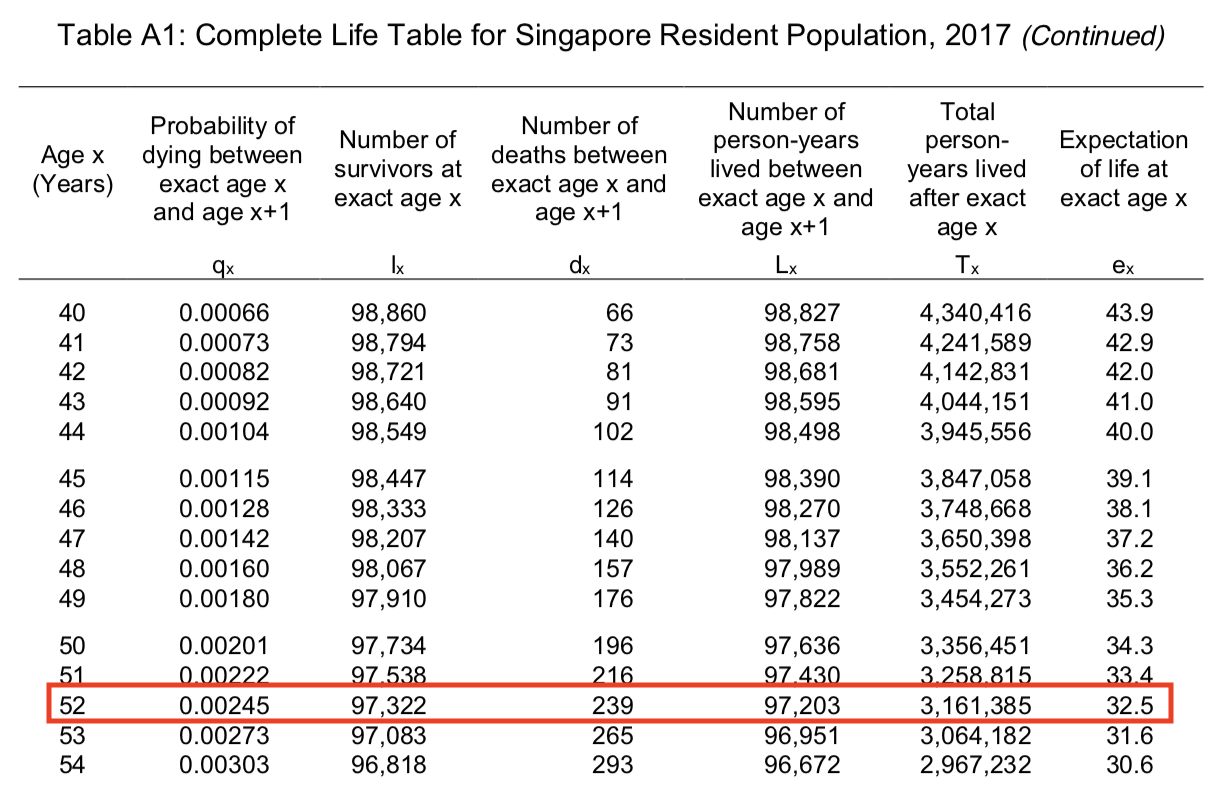
\includegraphics[width=0.8\linewidth]{images/apc/apc_lifetable2} 

}

\caption{Screenshot of Complete Life Table from the Department of Statistics. Retrieved September 17, 2019.}\label{fig:apc-lifetabletwo}
\end{figure}

Wait. We see now that those who aged 52 in 2017 can in fact expect to
live 32.5 more years. That means they are expected to live up to
\(52 + 32.5 = 84.5\) years old! That seems way different from the 64.5
years projected by mortality statistics in 1965. Why is this so? This is
because period life expectancy does not account for future improvements
in mortality driven by better healthcare, hygiene, health behaviors etc.
Period life expectancy is therefore often an \emph{underestimate} of the
true cohort life expectancy\footnote{Unless mortality rates spike due to
  events such as wars, famines etc.}. The discrepancy we see between the
1965 life table and the 2017 life table is likely due to great
improvements in mortality rates since independence.

Having studied how life expectancy `works', let us conclude by
evaluating this paragraph from an article on the
\href{https://dollarsandsense.sg/retirement-planning-singapore-live-beyond-average-life-expectancy/}{Dollars
and Sense website}, aimed at helping Singaporeans plan their retirement:

\begin{quote}
The next step of the retirement planning equation is to understand how
long we can expect to spend in retirement. The longer we spend in
retirement, the more we need to sustain ourselves.

\textbf{How Long Do We Spend In Retirement?} The simplest way to derive
this figure is to use the average life expectancy of Singaporeans --
which stands at 83.1 years today. This figure is only going to go up as
the latest report from the World Health Organisation (WHO) revealed that
people here can expect to live up to 85.4 years by 2040.

What this tells us is that if we retire at the moment we are able to
receive our CPF LIFE payouts -- at 65 -- and live to the average life
expectancy in Singapore -- to 83.1 -- we will have close to 18 years of
retirement.
\end{quote}

\textbf{What are the misinterpretations of life expectancy present
here?} First, the writer talks about average life expectancy as if it
applies to everyone. As we discussed, however, the number he uses likely
reflects the life expectancy \emph{at birth}. Is he speaking to newborns
and asking them to plan for retirement? A better approach would be to go
to the
\href{https://www.singstat.gov.sg/-/media/files/publications/population/lifetable17-18.pdf}{Complete
Life Tables} published by the Department of Statistics and refer to life
expectancy at 50 (or some other reference age that his target audience
can identify with). Second, he is correct that life expectancy will
probably continue to rise, but the 18 years (obtained supposedly using
\(83.1 - 65 \approx 18\)) is likely an underestimate of how long
``retirement'' will be (apart from the error already made in the first
point). Plan harder, people.

\section{Conclusion}\label{conclusion-3}

Age, period, and cohort effects are important ways to understand changes
in society over time. People most commonly mix up period and cohort
effects, such as offering cohort explanations for changes in period
measures, or mistaking one kind of change for the other. In many cases,
period and cohort rates tell the same overall story. Where they tend to
diverge is when there are large societal changes within short periods of
time (as in Singapore's case), as we have seen in the case of life
expectancy. Under such circumstances, period measures are usually bad
estimates of cohort change.

We often assume that experts and social scientists quoted in newspapers
are making statements about societal change based off empirical evidence
and research that they have done. But sometimes experts may just be
speculating about something there is no real data to show for (e.g., no
cohort data, and no research done to project cohort trends). In such a
case (and with the application of some common sense), anyone's
speculation may be as good as theirs. Where these speculations happily
coincide with reality they may be of some use, but readers should
carefully evaluate whether it is suitable for certain numbers to be used
to make certain points.

\chapter{Your case study}\label{case3}

\begin{verbatim}
Contributor: 
Date: 
\end{verbatim}

Another case study goes here. Do you wish to contribute? Send me an
email at
\href{mailto:shannon.ang@ntu.edu.sg}{\nolinkurl{shannon.ang@ntu.edu.sg}}

\bibliography{book.bib,packages.bib,rest.bib}


\end{document}
